\documentclass[12pt,a4paper]{article}

% --- Настройка языка и шрифтов для LuaLaTeX ---
\usepackage{fontspec}
\defaultfontfeatures{Ligatures=TeX,Scale=MatchLowercase}

\setmainfont{Alice-Regular}[
    Path=font/,
    Extension=.ttf,
    BoldFont = Alice-Regular,
    ItalicFont = Alice-Regular,
    BoldItalicFont = Alice-Regular,
    BoldFeatures = {FakeBold=1.6},
    ItalicFeatures = {FakeSlant=0.2},
    BoldItalicFeatures = {FakeBold=1.6,FakeSlant=0.2}
]

\newfontfamily\cyrillicfont{Alice-Regular}[
    Path=font/,
    Extension=.ttf,
    BoldFont = Alice-Regular,
    ItalicFont = Alice-Regular,
    BoldItalicFont = Alice-Regular,
    BoldFeatures = {FakeBold=1.6},
    ItalicFeatures = {FakeSlant=0.2},
    BoldItalicFeatures = {FakeBold=1.6,FakeSlant=0.2}
]

\usepackage{polyglossia}
\setmainlanguage{russian}
\setsansfont{TeX Gyre Heros}
\setmonofont{TeX Gyre Cursor}

\usepackage{graphicx}        					          % Графика
\usepackage[protrusion=false]{microtype}       	% Микротипографика
\usepackage{amsmath, amsfonts, amssymb, amsthm}	% Математика
\usepackage{braket} 							              % Braket нотация для квантовой механики
\usepackage{unicode-math} 						          % Современный пакет для математики в LuaLaTeX
\usepackage{longtable}       					          % Таблицы с разрывом страниц
\usepackage{tikz}           					          % Рисование
\usepackage[europeanresistors]{circuitikz}		  % Рисование электрических схем в европейском стиле
\usepackage{listings}							              % Для отображения кода
\usepackage{tabularx}       					          % Для таблиц во всю ширину
\usepackage{array}		  						            % Для расширенных возможностей таблиц
\usepackage{float}          					          % Для точного позиционирования фигур
\usepackage{pgfplots}                           % Для построения графиков
\usepackage{caption}                            % Для настройки подписей к рисункам и таблицам
\usepackage{xfp}                                % Для вычислений в LaTeX
\usepackage{luacode}                            % Для вставки Lua-кода
\pgfplotsset{compat=1.18}
\usepackage[a4paper,left=20mm,right=20mm,top=20mm,bottom=20mm]{geometry}

\usetikzlibrary{arrows.meta}

% --- Колонтитулы ---
\usepackage{fancyhdr}
\pagestyle{fancy}
\fancyhf{}

\renewcommand{\headrulewidth}{0.4pt}
\renewcommand{\footrulewidth}{0.4pt}
\renewcommand\lstlistingname{Исходный код}

\lstdefinestyle{main}{
	backgroundcolor=\color{gray!8},   
	commentstyle=\color{green!50!black},
	keywordstyle=\color{blue!80!black},
	numberstyle=\small\color{darkgray},
	stringstyle=\rmfamily\color{orange!90!black},
	basicstyle=\ttfamily\small,
	breakatwhitespace=false,         
	breaklines=true,                   
	keepspaces=true,                 
	numbers=left,                    
	numbersep=8pt,                  
	showspaces=false,                
	showstringspaces=false,
	showtabs=false,                  
	tabsize=4
}	

\lstset{style=main}

\newcolumntype{C}{>{\centering\arraybackslash}X}
\renewcommand{\arraystretch}{1.25}

% =========================================================
%         СЛУЖЕБНЫЕ КОМАНДЫ ДЛЯ ВЫЧИСЛЕНИЙ
% =========================================================
\newcommand{\CalcZero} [1]{\fpeval{round((#1),0)}}
\newcommand{\CalcOne}  [1]{\fpeval{round((#1),1)}}
\newcommand{\CalcTwo}  [1]{\fpeval{round((#1),2)}}
\newcommand{\CalcThree}[1]{\fpeval{round((#1),3)}}
\newcommand{\CalcFour} [1]{\fpeval{round((#1),4)}}
\newcommand{\CalcFive} [1]{\fpeval{round((#1),5)}}

\begin{luacode*}
-- Выборка измерений.
-- В Lua десятичная дробь пишется через точку, не через запятую.
E1data = { --- n = 100
  0.200675, 0.200678, 0.200670, 0.200661, 0.200661, 0.200656, 0.200654, 0.200656,
  0.200650, 0.200651, 0.200650, 0.200641, 0.200636, 0.200634, 0.200633, 0.200630,
  0.200637, 0.200659, 0.200659, 0.200649, 0.200644, 0.200643, 0.200648, 0.200650,
  0.200636, 0.200626, 0.200636, 0.200644, 0.200644, 0.200645, 0.200650, 0.200656,
  0.200647, 0.200639, 0.200639, 0.200646, 0.200653, 0.200644, 0.200633, 0.200643,
  0.200654, 0.200655, 0.200655, 0.200650, 0.200647, 0.200649, 0.200649, 0.200641,
  0.200647, 0.200645, 0.200638, 0.200630, 0.200628, 0.200625, 0.200631, 0.200646,
  0.200642, 0.200649, 0.200657, 0.200664, 0.200668, 0.200668, 0.200657, 0.200644,
  0.200650, 0.200646, 0.200638, 0.200647, 0.200649, 0.200645, 0.200662, 0.200665,
  0.200661, 0.200663, 0.200652, 0.200633, 0.200620, 0.200625, 0.200627, 0.200630,
  0.200630, 0.200630, 0.200633, 0.200631, 0.200636, 0.200635, 0.200625, 0.200630,
  0.200647, 0.200659, 0.200659, 0.200659, 0.200670, 0.200672, 0.200670, 0.200661,
  0.200657, 0.200664, 0.200665, 0.200663
}

E2R1data = { --- n = 102
  10.1325, 10.1324, 10.1324, 10.1324, 10.1324, 10.1324, 10.1324, 10.1324,
  10.1325, 10.1324, 10.1324, 10.1325, 10.1324, 10.1324, 10.1325, 10.1324,
  10.1324, 10.1324, 10.1324, 10.1324, 10.1324, 10.1324, 10.1324, 10.1325,
  10.1325, 10.1324, 10.1325, 10.1325, 10.1325, 10.1325, 10.1325, 10.1324,
  10.1325, 10.1325, 10.1325, 10.1324, 10.1324, 10.1325, 10.1324, 10.1324,
  10.1324, 10.1325, 10.1324, 10.1324, 10.1324, 10.1325, 10.1324, 10.1324,
  10.1324, 10.1324, 10.1324, 10.1324, 10.1324, 10.1324, 10.1324, 10.1324,
  10.1325, 10.1324, 10.1324, 10.1324, 10.1324, 10.1324, 10.1324, 10.1324,
  10.1324, 10.1324, 10.1324, 10.1324, 10.1324, 10.1324, 10.1324, 10.1324,
  10.1325, 10.1324, 10.1323, 10.1323, 10.1323, 10.1323, 10.1323, 10.1323,
  10.1323, 10.1324, 10.1323, 10.1323, 10.1323, 10.1323, 10.1323, 10.1323,
  10.1323, 10.1323, 10.1323, 10.1322, 10.1323, 10.1323, 10.1324, 10.1323,
  10.1323, 10.1323, 10.1323, 10.1323, 10.1323, 10.1323
}

E2R2data = { --- n = 100
  22.1109, 22.1108, 22.1108, 22.1108, 22.1109, 22.1107, 22.1107, 22.1107,
  22.1107, 22.1107, 22.1108, 22.1108, 22.1108, 22.1108, 22.1109, 22.1107,
  22.1108, 22.1108, 22.1108, 22.1108, 22.1108, 22.1108, 22.1108, 22.1108,
  22.1108, 22.1108, 22.1108, 22.1108, 22.1108, 22.1108, 22.1108, 22.1108,
  22.1107, 22.1108, 22.1107, 22.1108, 22.1108, 22.1108, 22.1108, 22.1108,
  22.1108, 22.1108, 22.1108, 22.1108, 22.1108, 22.1108, 22.1108, 22.1108,
  22.1108, 22.1108, 22.1108, 22.1108, 22.1109, 22.1108, 22.1109, 22.1108,
  22.1109, 22.1109, 22.1109, 22.1108, 22.1108, 22.1109, 22.1109, 22.1110,
  22.1110, 22.1111, 22.1110, 22.1111, 22.1110, 22.1110, 22.1110, 22.1110,
  22.1110, 22.1110, 22.1110, 22.1110, 22.1110, 22.1110, 22.1110, 22.1110,
  22.1110, 22.1110, 22.1110, 22.1110, 22.1110, 22.1110, 22.1110, 22.1110,
  22.1110, 22.1110, 22.1110, 22.1110, 22.1110, 22.1110, 22.1110, 22.1110,
  22.1110, 22.1110, 22.1110, 22.1110
}

E3data = { --- n = 101
  0.63556, 0.63552, 0.63553, 0.63553, 0.63545, 0.63545, 0.63540, 0.63541,
  0.63541, 0.63543, 0.63535, 0.63537, 0.63546, 0.63543, 0.63549, 0.63543,
  0.63538, 0.63547, 0.63544, 0.63541, 0.63540, 0.63543, 0.63544, 0.63546,
  0.63550, 0.63550, 0.63546, 0.63545, 0.63547, 0.63552, 0.63553, 0.63556,
  0.63554, 0.63551, 0.63553, 0.63558, 0.63556, 0.63550, 0.63552, 0.63546,
  0.63549, 0.63554, 0.63549, 0.63551, 0.63551, 0.63551, 0.63545, 0.63551,
  0.63552, 0.63553, 0.63547, 0.63551, 0.63546, 0.63549, 0.63554, 0.63549,
  0.63550, 0.63551, 0.63558, 0.63554, 0.63554, 0.63554, 0.63556, 0.63556,
  0.63559, 0.63552, 0.63554, 0.63550, 0.63551, 0.63556, 0.63561, 0.63560,
  0.63560, 0.63557, 0.63563, 0.63559, 0.63558, 0.63550, 0.63548, 0.63545,
  0.63543, 0.63545, 0.63542, 0.63543, 0.63548, 0.63551, 0.63555, 0.63557,
  0.63561, 0.63550, 0.63549, 0.63549, 0.63551, 0.63549, 0.63560, 0.63558,
  0.63559, 0.63562, 0.63561, 0.63557, 0.63557
}

function scale_array(array, factor)
    local result = {}

    for i, x in ipairs(array) do
        result[i] = x * factor
    end

    return result
end

function shift_array(array, shift)
    local result = {}

    for i, x in ipairs(array) do
        result[i] = x + shift
    end

    return result
end

function add_arrays(array1, array2)
  local result = {}
  local n1 = (type(array1) == "table") and #array1 or 0
  local n2 = (type(array2) == "table") and #array2 or 0
  local n = math.min(n1, n2)

  for i = 1, n do
    local a = (type(array1) == "table") and array1[i] or 0
    local b = (type(array2) == "table") and array2[i] or 0
    if type(a) ~= "number" then a = 0 end
    if type(b) ~= "number" then b = 0 end
    result[i] = a + b
  end

  return result
end

function multiply_arrays(array1, array2)
  local result = {}
  local n1 = (type(array1) == "table") and #array1 or 0
  local n2 = (type(array2) == "table") and #array2 or 0
  local n = math.min(n1, n2)

  for i = 1, n do
    local a = (type(array1) == "table") and array1[i] or 0
    local b = (type(array2) == "table") and array2[i] or 0
    if type(a) ~= "number" then a = 0 end
    if type(b) ~= "number" then b = 0 end
    result[i] = a * b
  end

  return result
end

-- Переводим данные из кОм в Омы
E2R1data = scale_array(E2R1data, 1000) 

-- Переводим данные из кОм в Омы
E2R2data = scale_array(E2R2data, 1000)

-- Создаём массив косвенных измерений для R
E2Rdata = add_arrays(E2R1data, E2R2data)

-- Функция для нахождения минимума в массиве.
function find_min(array)
    local min = array[1]

    for i, x in ipairs(array) do
        if x < min then
            min = x
        end
    end

    return min
end

-- Функция для нахождения максимума в массиве.
function find_max(array)
    local max = array[1]

    for i, x in ipairs(array) do
        if x > max then
            max = x
        end
    end

    return max
end

-- Функция для нахождения среднего значения в массиве.
function find_mean(array)
    local sum = 0

    for i, x in ipairs(array) do
        sum = sum + x
    end

    return sum / #array
end

-- Функция для нахождения медианы в массиве.
function find_median(array)
    local sorted = {}

    for i, x in ipairs(array) do
        sorted[i] = x
    end

    table.sort(sorted)

    if #sorted % 2 == 1 then
        return sorted[math.ceil(#sorted / 2)]
    else
        return (sorted[#sorted / 2] + sorted[#sorted / 2 + 1]) / 2
    end
end

-- Функция для нахождения дисперсии в массиве.
function find_variance(array)
    local mean = find_mean(array)
    local sum = 0

    for i, x in ipairs(array) do
        sum = sum + (x - mean)^2
    end

    return sum / (#array - 1)
end

-- Функция для нахождения стандартного отклонения в массиве.
function find_stddev(array)
    return math.sqrt(find_variance(array))
end

-- Функция для нахождения коэффициента куртозиса в массиве.
function find_kurtosis(array)
    local mean = find_mean(array)
    local stddev = find_stddev(array)
    local sum = 0

    for i, x in ipairs(array) do
        sum = sum + (x - mean)^4
    end

    return sum / (#array * stddev^4)
end

-- Функция для нахождения коэффициента асимметрии в массиве.
function find_skewness(array)
    local mean = find_mean(array)
    local stddev = find_stddev(array)
    local sum = 0

    for i, x in ipairs(array) do
        sum = sum + (x - mean)^3
    end

    return sum / (#array * stddev^3)
end

-- Функция подсчёта числа попаданий в интервал [left; right).
function count_in_interval(array, left, right)
    local count = 0

    for i, x in ipairs(array) do
        if x >= left and x < right then
            count = count + 1
        end
    end

    return count
end

-- Функция подсчёта числа попаданий в последний интервал [left; right].
function count_in_closed_interval(array, left, right)
    local count = 0

    for i, x in ipairs(array) do
        if x >= left and x <= right then
            count = count + 1
        end
    end

    return count
end

-- Вспомогательная функция: логарифм по основанию 2 (работает независимо от версии Lua)
function log2(x)
  return math.log(x) / math.log(2)
end

function Gamma(z)
  if z == 1 then
    return 1
  elseif z == 0.5 then
    return math.sqrt(math.pi)
  else
    return (z - 1) * Gamma(z - 1)
  end
end 

function t_dist_quantile(p, df)
  local x = math.sqrt(df * (1 - p) / p)
  local a = 4 * df - 1
  local b = x^2 + a^2
  local c = (x^2 * a^2) / b
  return math.sqrt(c)
end

-- Функция для генерации координат гистограммы под ybar interval.
-- ВАЖНО: ybar interval требует границы интервалов, а не центры.
function generate_histogram_interval_coords(array, n_intervals, x_min, x_max)
  local coords = {}
  local n = #array

  -- Защита от пустого массива
  if n == 0 then
    coords[1] = { x = 0, y = 0 }
    return coords
  end

  local mean = find_mean(array)
  local interval_width = (x_max - x_min) / n_intervals

  -- Защита от нулевой или невалидной ширины интервала
  if not (interval_width == interval_width) or interval_width == 0 then
    interval_width = 1e-12
  end

  local function is_finite(v)
    return v == v and v ~= math.huge and v ~= -math.huge
  end

  local MAX_COORD = 1e6
  local MAX_DENSITY = 1e9

  for i = 1, n_intervals do
    local left = x_min + (i - 1) * interval_width
    local right = x_min + i * interval_width
    local count

    if i == n_intervals then
      count = count_in_closed_interval(array, left, right)
    else
      count = count_in_interval(array, left, right)
    end

    local left_dev = left - mean
    if not is_finite(left_dev) then left_dev = 0 end
    if math.abs(left_dev) > MAX_COORD then
      left_dev = (left_dev > 0) and MAX_COORD or -MAX_COORD
    end

    local density = count / (n * interval_width)
    if not is_finite(density) then density = 0 end
    if math.abs(density) > MAX_DENSITY then
      density = (density > 0) and MAX_DENSITY or -MAX_DENSITY
    end

    coords[i] = { x = left_dev, y = density }
  end

  -- Правая граница последнего интервала
  local last_x = x_max - mean
  if not is_finite(last_x) then last_x = 0 end
  if math.abs(last_x) > MAX_COORD then last_x = (last_x > 0) and MAX_COORD or -MAX_COORD end
  coords[#coords + 1] = { x = last_x, y = 0 }

  return coords
end

-- =========================
-- Плотности распределений
-- =========================

function normal_pdf(x, mu, sigma)
    return
        1 / (sigma * math.sqrt(2 * math.pi))
        * math.exp(-0.5 * ((x - mu) / sigma)^2)
end

function uniform_pdf(x, a, b)
    if x >= a and x <= b then
        return 1 / (b - a)
    else
        return 0
    end
end

-- =========================
-- Критерий хи-квадрат Пирсона
-- =========================
-- distribution:
-- "normal"  -- нормальное распределение
-- "uniform" -- равномерное распределение

function pearson_chi_square(array, r, distribution, m, S)
    local n = #array
    local x_min = find_min(array)
    local x_max = find_max(array)
    local l = (x_max - x_min) / r

    local chi_square = 0
    local rows = {}

    for j = 1, r do
        local left = x_min + (j - 1) * l
        local right = x_min + j * l

        local O_j

        if j < r then
            O_j = count_in_interval(array, left, right)
        else
            right = x_max
            O_j = count_in_closed_interval(array, left, right)
        end

        local x0_j = (left + right) / 2
        local E_j

        if distribution == "normal" then
            E_j = n * l * normal_pdf(x0_j, m, S)
        elseif distribution == "uniform" then
            -- Для равномерного распределения на [x_min; x_max]
            -- при равных интервалах ожидаемое число попаданий одинаковое:
            E_j = n / r

            -- Эквивалентная запись:
            -- E_j = n * l * uniform_pdf(x0_j, x_min, x_max)
        else
            error("Неизвестное распределение: " .. tostring(distribution))
        end

        local chi_j = 0

        if E_j > 0 then
            chi_j = (O_j - E_j)^2 / E_j
            chi_square = chi_square + chi_j
        else
            error("E_j = 0 в интервале " .. j)
        end

        rows[#rows + 1] = {
            j = j,
            left = left,
            right = right,
            center = x0_j,
            observed = O_j,
            expected = E_j,
            chi = chi_j
        }
    end

    return chi_square, rows
end

-- безопасная версия value_with_mantice
local function round_fallback(x)
  if x >= 0 then return math.floor(x + 0.5) else return math.ceil(x - 0.5) end
end
local round = math.round or round_fallback

function value_with_mantice(value, precision, shift, scale)
  precision = precision or 5
  shift = shift or 0
  scale = scale or 0

  if value == nil or value ~= value then
    return "\\fpeval{0}"
  end
  if value == 0 then
    return "\\fpeval{0}"
  end

  local sign = ""
  if value < 0 then
    sign = "-"
    value = math.abs(value)
  end

  local logv = math.log10(value)
  if not (logv == logv) then -- проверка на NaN
    return "\\fpeval{0}"
  end

  local floorlog = math.floor(logv)
  local mantissa = round(value * 10^(precision - 1 - floorlog)) * 10^(-(precision - 1) + shift - scale)
  local exponent = floorlog - shift

  if exponent == 0 then
    return sign .. "\\fpeval{" .. mantissa .. "}"
  else
    return sign .. "\\fpeval{" .. mantissa .. "} \\cdot 10^{" .. exponent .. "}"
  end
end

-- Сопротивление резистора генератора
R_G = 50
-- Сопротивление входа мультиметра
R_M = 100000000
-- Критерий Хи-квадрат для 5% уровня значимости и 4 степенями свободы 
chi2critical = 9.49
-- Theta_U = 0.015% от измеряемой величины + 0.003% от измеряемой величины
-- Theta_R = 0.020% от измеряемой величины + 0.003% от измеряемой величины


-- Данные для определения поправки
n1 = #E1data
t1 = 1.984216951586419
r1 = 1 + math.floor(log2(n1))
m1 = find_mean(E1data)

-- Вводим поправку 
E1data = shift_array(E1data, m1 * (R_G / R_M)) 

-- Данные после поправки
m11 = find_mean(E1data)
D1 = find_variance(E1data)
S1 = find_stddev(E1data)
k1 = find_kurtosis(E1data)
A1 = find_skewness(E1data)

-- Хистограма
E1histogram_interval_coords = generate_histogram_interval_coords(E1data, r1, find_min(E1data), find_max(E1data))

chi21 = pearson_chi_square(E1data, r1, "normal", m11, S1)

-- Вычисление погрешности
Sm1 = S1 / math.sqrt(n1)
delta_m11 = t1 * Sm1
Theta1 = 0.015 * m11 / 100 + 0.003 * 2 / 100
Stheta1 = Theta1 / math.sqrt(3)
K1 = (delta_m11 + Theta1) / (Sm1 + Stheta1)
Ssum1 = math.sqrt(Sm1^2 + Stheta1^2)
delta1 = K1 * Ssum1

n2 = #E2R1data
r2 = 1 + math.floor(log2(n2))
m2 = find_mean(E2R1data)

E2R1data = shift_array(E2R1data, 0.2) -- Вводим поправку

m21 = find_mean(E2R1data)
D2 = find_variance(E2R1data)
S2 = find_stddev(E2R1data)
k2 = find_kurtosis(E2R1data)
A2 = find_skewness(E2R1data)

-- Построение гистограммы для R1 в кОм: масштабируем массив корректно
E2R1histogram_interval_coords = generate_histogram_interval_coords(scale_array(E2R1data, 10^(-3)), r2, find_min(E2R1data) * 10^(-3), find_max(E2R1data) * 10^(-3))

-- Сравниваем в тех же единицах (кОм): передаём min/max и S в кОм
chi22 = pearson_chi_square(scale_array(E2R1data, 10^(-3)), r2, "normal", m21 * 10^(-3), S2 * 10^(-3))

Sm2 = S2 / math.sqrt(n2)
delta_m21 = Sm2 / (math.sqrt(0.05) * math.sqrt(n2))
Theta2 = 0.020 * m21 / 100 + 0.003 * 20000 / 100
Stheta2 = Theta2 / math.sqrt(3)
K2 = (delta_m21 + Theta2) / (Sm2 + Stheta2)
Ssum2 = math.sqrt(Sm2^2 + Stheta2^2)
delta2 = K2 * Ssum2

n3 = #E2R2data
r3 = 1 + math.floor(log2(n3))
m3 = find_mean(E2R2data)

E2R2data = shift_array(E2R2data, 0.2) -- Вводим поправку

m31 = find_mean(E2R2data)
D3 = find_variance(E2R2data)
S3 = find_stddev(E2R2data)
k3 = find_kurtosis(E2R2data)
A3 = find_skewness(E2R2data)

E2R2histogram_interval_coords = generate_histogram_interval_coords(scale_array(E2R2data, 10^(-3)), r3, find_min(E2R2data) * 10^(-3), find_max(E2R2data) * 10^(-3))

chi23 = pearson_chi_square(scale_array(E2R2data, 10^(-3)), r3, "normal", m31 * 10^(-3), S3 * 10^(-3))

Sm3 = S3 / math.sqrt(n3)
delta_m31 = Sm3 / (math.sqrt(0.05) * math.sqrt(n3))
Theta3 = 0.020 * m31 / 100 + 0.003 * 200000 / 100
Stheta3 = Theta3 / math.sqrt(3)
K3 = (delta_m31 + Theta3) / (Sm3 + Stheta3)
Ssum3 = math.sqrt(Sm3^2 + Stheta3^2)
delta3 = K3 * Ssum3

n4 = #E2Rdata
z4 = 1.96
m4 = m21 + m31
Sm4 = math.sqrt(Sm2^2 + Sm3^2)
Theta4 = math.sqrt(Theta2^2 + Theta3^2)

delta_m41 = z4 * Sm4
Stheta4 = Theta4 / math.sqrt(3)
K4 = (delta_m41 + Theta4) / (Sm4 + Stheta4)
Ssum4 = math.sqrt(Sm4^2 + Stheta4^2)
delta4 = K4 * Ssum4

n5 = #E3data
t5 = 1.9840
r5 = 1 + math.floor(log2(n5))
m5 = find_mean(E3data)
D5 = find_variance(E3data)
S5 = find_stddev(E3data)
k5 = find_kurtosis(E3data)
A5 = find_skewness(E3data)

E3histogram_interval_coords = generate_histogram_interval_coords(E3data, r5, find_min(E3data), find_max(E3data))

chi25 = pearson_chi_square(E3data, r5, "normal", m5, S5)

Sm5 = S5 / math.sqrt(n5)
delta_m5 = t5 * Sm5
Theta5 = 0.015 * m5 / 100 + 0.003 * 2 / 100
Stheta5 = Theta5 / math.sqrt(3)
K5 = (delta_m5 + Theta5) / (Sm5 + Stheta5)
Ssum5 = math.sqrt(Sm5^2 + Stheta5^2)
delta5 = K5 * Ssum5

-- Косвенная оценка выходного напряжения измерительного преобразователя 
n6 = math.min(n1, n2, n3) 
z6 = 1.96 

dUdU6 = 1 + m31 / m21 
dUdR16 = -m11 * m31 / (m21^2) 
dUdR26 = m11 / m21 

m6 = (1 + m31 / m21) * m11 

Sm6 = math.sqrt((dUdU6 * Sm1)^2 + (dUdR16 * Sm2)^2 + (dUdR26 * Sm3)^2) 
Theta6 = math.sqrt((dUdU6 * Theta1)^2 + (dUdR16 * Theta2)^2 + (dUdR26 * Theta3)^2) 

delta_m6 = z6 * Sm6 
Stheta6 = Theta6 / math.sqrt(3) 
K6 = (delta_m6 + Theta6) / (Sm6 + Stheta6) 
Ssum6 = math.sqrt(Sm6^2 + Stheta6^2) 
delta6 = K6 * Ssum6 

U1min = m11 - delta1
U1max = m11 + delta1

R1min = m21 - delta2
R1max = m21 + delta2

R2min = m31 - delta3
R2max = m31 + delta3

RsumMin = m4 - delta4
RsumMax = m4 + delta4

UoutDirectMin = m5 - delta5
UoutDirectMax = m5 + delta5

UoutIndirectMin = m6 - delta6
UoutIndirectMax = m6 + delta6

UoutIntervalsCross =
  math.max(UoutDirectMin, UoutIndirectMin) <= math.min(UoutDirectMax, UoutIndirectMax)


\end{luacode*}

% ---------------------------------------------------------
% ОБЩИЕ ДАННЫЕ
% ---------------------------------------------------------
\def\VariantN{4}          					  % Номер варианта
\def\LabNumber{3}							        % Номер лабораторной работы
\def\Discipline{Метрология}				    % Название дисциплины
\def\LabTitle{Многократные измерения}	% Название лабораторной работы

\title{
	МИНОБРНАУКИ РОССИИ

	федеральное государственное автономное образовательное учреждение

	высшего образования

	«Национальный исследовательский университет
	«Московский институт электронной техники»
	\vspace{2em}
}
\author{
}
\date{}

\begin{document}

\maketitle
\thispagestyle{fancy}

\begin{center}
\Large Отчёт по Лабораторной работе $\LabNumber$\\
по дисциплине «\Discipline»\\
«\LabTitle»
\end{center}

\begin{center}
\Large Вариант \VariantN
\end{center}

\vspace{12em}

\begin{flushright}
	Выполнили студенты группы ЭН-$25$\\
	Андреев И. А.\\
	Анисимов А. С.\\
  и ЭН-$21$ \\ 
  Рыжов Р. Р.\\
	Проверил преподаватель\\
	Туринцев К. А.
\end{flushright}

\cfoot{Москва 2026}

\pagebreak

\fancyhead[L]{\LabTitle} 
\fancyhead[R]{\Discipline}
\fancyfoot[C]{\thepage}


\pagebreak
\fancyhead[L]{Оглавление}
\fancyhead[R]{\LabTitle}
\fancyfoot[C]{\thepage}
\tableofcontents
\pagebreak

\fancyhead[L]{Теория}
\fancyhead[R]{\LabTitle}

\begin{center}
\Large\textbf{Лабораторная работа $\LabNumber$}
\end{center}

\begin{center}
\LARGE\textbf{\LabTitle}
\end{center}

\large\textbf{\textit{Цель работы}:} постановка многократных прямых и косвенных измерений 
и оценка действительных значений измеряемых величин с последующей 
оценкой погрешностей данных измерений.

\large\textbf{\textit{Необходимое оборудование}:} цифровой мультиметр 
(\textbf{Rigol DM$3058$}), генератор сигналов (\textbf{Rigol DG$1022$Z}), макетная плата, 
кабели, перемычки, щупы.

\fancyhead[L]{Теория}
\section{Теоретические сведения}

Многократные измерения позволяют получить более достоверную
оценку измеряемой величины и являются важным инструментом для
оценки случайной погрешности.

\textbf{Случайная погрешность} – составляющая погрешности измерения,
изменяющаяся случайным образом (по знаку и значению) при повторных измерениях, 
произведенных в определенных условиях. Случайные
погрешности легко обнаруживаются, однако, в отличие от систематических 
погрешностей, на случайные погрешности невозможно ввести поправку, 
поскольку они изменяются непредсказуемо и не имеют постоянного характера, 
т. е. являются случайной величиной.

\textbf{Промах} – результат измерения, который сильно отклоняется от основной массы значений 
и не соответствует ожидаемому распределению.

При статических измерениях каждое значение выборки содержит в
себе как реализацию случайной погрешности $\sigma$, так и систематическую
погрешность $\theta$
\begin{equation}
x_i = \mu + \theta + \sigma_i = \mu + \Delta_i
\tag{0.1}
\end{equation}
где $\mu$ – истинное значение измеряемой величины, $\theta$ – систематическая 
погрешность, $\sigma_i$ – случайная погрешность $i$-го измерения. При многократных 
измерениях систематическая погрешность $\theta$ остается постоянной, в то время как 
случайная погрешность $\sigma_i$ изменяется от измерения к измерению.

\subsection{Гистограмма экспериментального распределения и гипотетическое распределение}

Для гистограммы необходимо выбрать оптимальное количество интервалов
\begin{equation}
r = 1 + \lfloor \log_2 n \rfloor
\tag{1.1}
\label{gistogram:r}
\end{equation}
где $n$ – количество измерений. Гистограмма позволяет визуально оценить форму
распределения данных и выявить наличие выбросов.

Ширина интервала гистограммы определяется по формуле
\begin{equation*}
l = \frac{x_{max} - x_{min}}{r}
\end{equation*}

после чего необходимо выявить наблюдаемое число попаданий $N_i$ в каждый интервал 
$L_i = [x_{min} + (i-1)l, x_{min} + il]$, также желательно построить теоретическую кривую
гипотетического распределения

Когда предполагается, что данные подчиняются \textbf{нормальному распределению}, плотность 
вероятности может быть описана формулой

\begin{equation}
f(x) = \frac{1}{\sigma \sqrt{2\pi}} e^{-\frac{1}{2}\left(\frac{x - \mu}{\sigma}\right)^2}
\tag{1.2}
\label{normal_distribution}
\end{equation}
где $\mu$ – математическое ожидание, $\sigma$ – среднеквадратическое отклонение.

В качестве точечной оценки математического ожидания $\mu$ можно использовать выборочное среднее
\begin{equation}
\tilde{\mu} = \overline{x} = \frac{1}{n} \sum_{i=1}^{n} x_i
\tag{1.3}
\label{normal_distribution:mean}
\end{equation}

В качестве точечной оценки среднеквадратического отклонения $\overline{\sigma}$ можно 
использовать выборочное стандартное отклонение
\begin{equation}
\tilde{\sigma} = \sqrt{\frac{1}{n-1} \sum_{i=1}^{n} (x_i - \overline{x})^2}
\tag{1.4}
\label{normal_distribution:stddev}
\end{equation}

В качестве точечной оценки среднеквадратического отклонения $\overline{\sigma}_{\overline{x}}$ можно 
использовать выборочное стандартное отклонение
\begin{equation}
\tilde{\sigma}_{\overline{x}} = \frac{\tilde\sigma}{\sqrt{n}} = \sqrt{\frac{1}{n(n-1)} \sum_{i=1}^{n} (x_i - \overline{x})^2}
\tag{1.5}
\label{normal_distribution:stddev:mean}
\end{equation}

Когда предполагается, что данные подчиняются \textbf{равномерному распределению}, плотность 
вероятности может быть описана формулой
\begin{equation*}
f(x) = \begin{cases}
\displaystyle\frac{1}{b - a} & a \leq x \leq b \\
0 & \text{иначе}
\end{cases}
\end{equation*}
где $a$ и $b$ – границы равномерного распределения
\begin{equation*}
a = \min(x_i), \quad b = \max(x_i)
\end{equation*} 

В этом случае точечной оценкой для математического ожидания $\mu$ может служить 
середина интервала $[a, b]$
\begin{equation}
\tilde{\mu} = \frac{a + b}{2}
\tag{1.6}
\end{equation}

В качестве точечной оценки среднеквадратического отклонения $\overline{\sigma}$ можно 
использовать формулу
\begin{equation}
\tilde{\sigma} = \frac{b - a}{2\sqrt{3}}
\tag{1.7}
\end{equation}

Если расспределение данных не известно, то для оценки математического ожидания $\mu$ 
можно использовать критерий 
\begin{equation}
  \kappa = \frac{\displaystyle\sum_{i=1}^{n} (x_i - \overline{x})^4}{n\tilde{\sigma}^4}
\tag{1.8}
\label{kurtosis}
\end{equation}

\begin{itemize}
  \item $1.8 \le \kappa < 2.5$: мат ожидание $\mu$ оценивается как середина интервала
  \begin{equation*}
    \tilde{q} = \frac{x_{\min} + x_{\max}}{2} 
  \end{equation*}
  \item $2.5 \le \kappa < 4$: мат ожидание $\mu$ оценивается как выборочное среднее
  \begin{equation*}
    \tilde{q} = \frac{1}{n} \sum_{i=1}^{n} x_i 
  \end{equation*}
  \item $\kappa \ge 4$: мат ожидание $\mu$ оценивается как медиана выборки
  \begin{equation*}
    \tilde{q} = \begin{cases}
      \frac{1}{2}\left(x_{\frac{n}{2}} + x_{\frac{n}{2} + 1}\right) & n = \text{чётное} \\
      x_{\frac{n+1}{2}} & n = \text{нечётное}
    \end{cases}
  \end{equation*}
\end{itemize}

Также заметим, что коэффициент куртозиса $\kappa$ для нормального распределения равен 
$3$, для равномерного распределения равен $1.8$. Отсюда коэффициент эксцесса  
\begin{equation}
  \mathcal{K} = \kappa - 3
  \tag{1.9}
\end{equation}
это нормированный показатель остроконечности распределения

Коэффициент асимметрии $\mathcal{A}$ для нормального распределения равен $0$, для равномерного распределения 
равен $0$. Считается в свою очередь по формуле
\begin{equation}
  \mathcal{A} = \frac{\displaystyle\sum_{i=1}^{n} (x_i - \overline{x})^3}{n\tilde{\sigma}^3}
  \tag{1.10}
\end{equation}
это нормированный показатель асимметрии распределения

\subsection{Оценка промахов}

Метод трёх сигм — выкидывается каждое значение, которое отклоняется от среднего более чем на три стандартных отклонения
\begin{equation}
|x_i - \overline{x}| > 3\tilde{\sigma}
\tag{2}
\label{3sigma}
\end{equation}

\subsection{Оценка гипотезы о виде распределения}

Можно использовать критерий $\chi^2$ Пирсона. Для этого необходимо разбить данные на интервалы, подсчитать наблюдаемое число попаданий $N_i$ в каждый интервал $L_i$, а также вычислить теоретическое число попаданий $N_i^{(t)}$ в каждый интервал, используя формулу
\begin{equation}
N_i^{(t)} = nlf(x_{i0})
\tag{3.1}
\end{equation}
где $f(x)$ – плотность вероятности соответствующего распределения. Затем необходимо вычислить значение статистики $\chi^2$ по формуле
\begin{equation}
\chi^2 = \sum_{i=1}^{r} \frac{\left(N_i - N_i^{(t)}\right)^2}{N_i^{(t)}}
\tag{3.2}
\end{equation}

После чего необходимо сравнить полученное значение $\chi^2$ с критическим значением 
$\chi^2_{q,\,\nu}$ для уровня значимости $q = 1 - \alpha$ и количества степеней свободы $\nu = r - s - 1$, 
где $s$ – количество параметров распределения, оцененных по данным.
\begin{equation}
  P\left(\chi^2 > \chi^2_{q,\,\nu}\right) = q 
  \qquad
  q =
  \frac{1}{2^{\nu/2}\Gamma(\nu/2)}
  \int\limits_{\chi^2_{q,\,\nu}}^{+\infty}
  x^{\nu/2 - 1} e^{-x/2}\,dx
  \tag{3.3}
  \label{chi2:critical}
\end{equation}

Если $\chi^2 < \chi^2_{q,\,\nu}$, то гипотеза о виде распределения не отвергается.

\subsection{Оценка доверительной погрешности величины}

Если известно, что данные подчиняются нормальному распределению, то для оценки 
доверительной погрешности можно использовать распределение Стьюдента
\begin{equation*}
  t = \frac{\overline{x} - \mu}{\tilde{\sigma}_{\overline{x}}}
\end{equation*}
откуда можно получить критерий Стьюдента для оценки доверительной погрешности
\begin{equation}
  \varepsilon(\alpha) = \pm t_{q,\,\nu}\tilde{\sigma}_{\overline{x}} \qquad \nu = n - 1
  \tag{4.1}
  \label{student:confidence}
\end{equation}
где $t_{q,\,\nu}$ – квантиль распределения Стьюдента для уровня значимости $q = \\ = 1 - \alpha$ и 
количества степеней свободы $\nu = n - 1$
\begin{equation}
  P\left(t > t_{q,\,\nu}\right) = 1 - \frac{q}{2}
  \qquad
  1 - \frac{q}{2} = \int\limits_{-\infty}^{t_{q,\,\nu}}
  \frac{\Gamma(\frac{\nu + 1}{2})}{\sqrt{\pi\nu}\Gamma(\frac{\nu}{2})}
  \left(1 + \frac{x^2}{\nu}\right)^{-\frac{\nu + 1}{2}}\,dx
  \tag{4.2}
  \label{student:critical}
\end{equation}

Если же распределение данных не является нормальным, но с определённой дисперсией, то 
для оценки доверительной погрешности можно использовать неравенство Чебышёва
\begin{equation*}
  \varepsilon(\alpha) = \pm t_{q}\frac{\tilde{\sigma}}{\sqrt{n}} \qquad t_{q} = \frac{1}{\sqrt{q}}
  \tag{4.3}
  \label{chebyshev:confidence}
\end{equation*}

Но при равномерном распределении данных лучше использовать формулу полуразмаха
\begin{equation*}
  \varepsilon(\alpha) = \pm \frac{x_{\max} - x_{\min}}{2}\alpha
\end{equation*}

Для оценки суммарной неисключаемой систематической погрешности при двух членах можно 
использовать формулу
\begin{equation}
  \Theta_\Sigma = \pm\left(\left|\Theta_1\right| + \left|\Theta_2\right|\right)
  \tag{4.4}
\end{equation}
при большем количестве членов можно использовать формулу
\begin{equation}
  \Theta_\Sigma = \pm k_\alpha\sqrt{\Theta_1^2 + \Theta_2^2 + \ldots + \Theta_i^2}
  \tag{4.5}
\end{equation}
где $k_{0.95} = 1.1$.

Погрешность оценки измеряемой величины $\tilde{q}$ можно оценить по формуле
\begin{equation}
  \Delta(\alpha) = \pm K\tilde{\sigma}_\Sigma \quad K = \frac{\varepsilon(\alpha) + \Theta_\Sigma}{\tilde{\sigma}_\Theta + \tilde{\sigma}_{\overline{x}}} \quad \tilde{\sigma}_\Sigma = \sqrt{\tilde{\sigma}_\Theta^2 + \tilde{\sigma}_{\overline{x}}^2}
  \tag{4.6}
  \label{delta:confidence}
\end{equation}
отсюда 
\begin{equation*}
  \tilde{\sigma}_\Theta = \frac{\Theta_\Sigma}{\sqrt{3}} \qquad \tilde{\sigma}_\Theta = \frac{\Theta_\Sigma(\alpha)}{k_\alpha\sqrt{3}}
\end{equation*}

Согласно ГОСТу измерение положено записывать с учётом значащих цифр
\begin{equation}
  q = \tilde{q} \pm \Delta(\alpha) 
  \tag{4.7}
  \label{final:result}
\end{equation}

\subsection{Оценка доверительной погрешности косвенных измерений}

Косвенные измерения — измерения, при которых искомое значение
величины определяют на основании результатов прямых измерений
других величин, функционально связанных с искомой величиной.

Линейные косвенные измерения описываются формулой
\begin{equation}
  y = b_1 x_1 + b_2 x_2 + \ldots + b_m x_m
  \tag{5.1}
  \label{linear:indirect}
\end{equation}
где $x_i$ – результат прямого измерения, $b_i$ – коэффициент пропорциональности.

Оценка результата линейного косвенного измерения, так же как и
прямых измерений, – это оценка математического ожидания данной
величины
\begin{equation*}
  \tilde{y} = b_1 \tilde{x}_1 + b_2 \tilde{x}_2 + \ldots + b_m \tilde{x}_m
  \tag{5.2}
  \label{linear:indirect:result}
\end{equation*}

Погрешность косвенного измерения может быть оценена по формуле
\begin{equation*}
  \tilde{y} = \sum_{i=1}^{m} b_i (\mu_i + \Delta_i)
\end{equation*}

Если измерения аргументов проводились в разное время и так как связь
между ними линейна, то
\begin{equation*}
  \tilde{\sigma}_{\tilde{y}} = \sqrt{\sum_{i=1}^{m} b_i^2 \tilde{\sigma}_{x_i}^2}
  \tag{5.3}
  \label{linear:indirect:stddev}
\end{equation*}

Доверительная погрешность косвенного измерения может быть оценена по формуле
\begin{equation*}
  \varepsilon_{y}(\alpha) = \pm z_{\frac{1+\alpha}{2}} \tilde{\sigma}_{\tilde{y}}
  \tag{5.4}
  \label{linear:indirect:confidence}
\end{equation*}

Суммарная неисключаемая систематическая погрешность косвенного измерения может быть оценена
как
\begin{equation*}
  \Theta_{y}(\alpha) = \sqrt{\sum_{i=1}^{m} b_i^2 \Theta_{x_i}^2(\alpha)}
  \tag{5.5}
  \label{linear:indirect:systematic}
\end{equation*}

Если косвенные измерения описываются нелинейной формулой, то необходимо линеризовать  
косвенную зависимость. Для линеаризации необходимо разложить исходную функцию в
ряд Тейлора с исключением всех элементов ряда дальше первого, что
можно сделать только после оценки остаточного члена разложения – он
не должен превышать погрешности аргументов. При определенных
ограничениях точечная оценка СКО, доверительная граница случайной
погрешности и общей НСП нелинейного косвенного измерения устанавливаются 
следующими формулами
\begin{equation*}
  \tilde{\sigma}_{\tilde{y}} = \sqrt{\sum_{i=1}^{m} \left(\frac{\partial f}{\partial x_i}\right)^2 \tilde{\sigma}_{x_i}^2} \quad \varepsilon_{y}(\alpha) = \pm z_{\frac{1+\alpha}{2}} \tilde{\sigma}_{\tilde{y}} \quad \Theta_{y}(\alpha) = \sqrt{\sum_{i=1}^{m} \left(\frac{\partial f}{\partial x_i}\right)^2 \Theta_{x_i}^2(\alpha)}
  \tag{5.6}
  \label{nonlinear:indirect}
\end{equation*}

Доверительные границы погрешности оценки косвенно измеряемой величины вычисляются 
как для прямых измерений
\begin{equation*}
  \Delta_{\tilde{y}}(\alpha) = \pm K \tilde{\sigma}_\Sigma \qquad K = \frac{\varepsilon_{y}(\alpha) + \Theta_{y}(\alpha)}{\tilde{\sigma}_\Theta + \tilde{\sigma}_{\tilde{y}}} \qquad \tilde{\sigma}_\Sigma = \sqrt{\tilde{\sigma}_\Theta^2 + \tilde{\sigma}_{\tilde{y}}^2}
  \tag{5.7}
  \label{nonlinear:indirect:confidence}
\end{equation*}
отсюда
\begin{equation*}
  \tilde{\sigma}_\Theta = \frac{\Theta_{y}(\alpha)}{k_\alpha\sqrt{3}}
\end{equation*}

\subsection{Масштабирующий измерительный преобразователь на базе операционного усилителя}

На рис. \ref{fig:scheme1} представлена схема масштабирующего измерительного
преобразователя на основе операционного усилителя (ОУ), работающего в 
режиме неинвертирующего усиления. Входной сигнал поступает на
неинвертирующий вход ОУ и увеличивается пропорционально коэффициенту 
усиления, который определяется отношением сопротивлений
резисторов $R_1$ и $R_2$, включенных в обратную связь усилителя.

\begin{figure}[H]
  \centering
  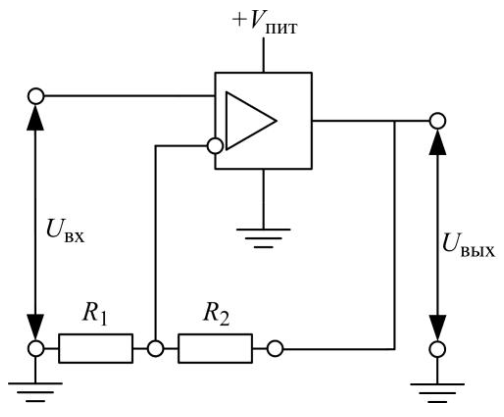
\includegraphics[width=0.5\textwidth]{scheme1.png}
  \caption{Масштабирующий измерительный преобразователь на базе операционного усилителя}
  \label{fig:scheme1}
\end{figure}

Выходное напряжение 
\begin{equation*}
  U_\text{вых} = \left(1 + \frac{R_2}{R_1}\right) U_\text{вх}
  \tag{6.1}
  \label{amplifier:output}
\end{equation*}
Коэффициент усиления
\begin{equation*}
  K = 1 + \frac{R_2}{R_1}
  \tag{6.2}
  \label{amplifier:gain}
\end{equation*}
Погрешность усиления
\begin{equation*}
  \Delta K = \frac{R_2\Delta R_1 + R_1\Delta R_2}{R_1^2}
  \tag{6.3}
  \label{amplifier:gain:uncertainty}
\end{equation*}

\pagebreak

\begin{center}
\LARGE{\textbf{Выполнение лабораторной работы и расчетно-графическая часть}}
\end{center}

Выполнятся работа будет для доверительного уровня $\alpha = 0.95$.

Выборки содержат примерно по $n \approx 100$ элементов каждая, поэтому оптимальное количество интервалов для
гистограммы считаем по формуле (\ref{gistogram:r})
\begin{equation*}
  r = 1 + \lfloor \log_2 100 \rfloor = 1 + 6 = 7
\end{equation*}

Ищем коэффициент $\chi_{q, \nu}^2$ для $q = 1 - \alpha = 0.05$ и $\nu = r - s - 1 = 4$ степеней свободы по
формуле (\ref{chi2:critical})
\begin{equation*}
  \begin{aligned}
    & 0.05 = \frac{1}{2^{4/2}\Gamma(4/2)} \int\limits_{\chi^2_{0.05, 4}}^{+\infty} x^{4/2 - 1} e^{-x/2}\,dx \iff 0.05 = \frac{1}{4} \int\limits_{\chi^2_{0.05, 4}}^{+\infty} x e^{-x/2}\,dx \iff \\
    & \iff 0.05 = -\frac{2}{4}\left(x e^{-x/2}\Big|_{\chi^2_{0.05, 4}}^{+\infty} - \int\limits_{\chi^2_{0.05, 4}}^{+\infty} e^{-x/2}\,dx \right) \iff \\
    & \iff - 0.1 = \left(-\chi^2_{0.05, 4} - 2\right) e^{-\chi^2_{0.05, 4}/2} \iff \left(\chi^2_{0.05, 4} + 2\right) e^{-\chi^2_{0.05, 4}/2} = 0.1
  \end{aligned}
\end{equation*}
Корни ищем численно, будет 
\begin{equation*}
  \chi^2_{0.05, 4} \approx 9.49
\end{equation*}

Ищем коэффициент $t_{q, \nu}$ для $q = 1 - \alpha = 0.05$ и $\nu = n - 1 = \directlua{tex.print(n1 - 1)}$ степеней свободы по 
формуле (\ref{student:critical})
\begin{equation*}
  \begin{aligned}
    & 0.05 = \int\limits_{t_{0.05, \directlua{tex.print(n1 - 1)}}}^{+\infty} \frac{\Gamma(\frac{\directlua{tex.print(n1 - 1)} + 1}{2})}{\sqrt{\pi \cdot \directlua{tex.print(n1 - 1)}}\Gamma(\frac{\directlua{tex.print(n1 - 1)}}{2})} \left(1 + \frac{x^2}{\directlua{tex.print(n1 - 1)}}\right)^{-\frac{\directlua{tex.print(n1 - 1)} + 1}{2}}\,dx \iff  \\ 
    & \iff 0.05 = \CalcFive{\directlua{tex.print((Gamma(((n1 - 1) + 1) / 2) / (math.sqrt((n1 - 1) * math.pi) * Gamma((n1 - 1) / 2))))}}\int\limits_{t_{0.05, \directlua{tex.print(n1 - 1)}}}^{+\infty} \left(1 + \frac{x^2}{\directlua{tex.print(n1 - 1)}}\right)^{-\frac{\directlua{tex.print(n1 - 1)} + 1}{2}}\,dx \iff \\
    & \iff \CalcFive{\directlua{tex.print(0.05/(Gamma(((n1 - 1) + 1) / 2) / (math.sqrt((n1 - 1) * math.pi) * Gamma((n1 - 1) / 2))))}} = \int\limits_{t_{0.05, \directlua{tex.print(n1 - 1)}}}^{+\infty} \left(1 + \frac{x^2}{\directlua{tex.print(n1 - 1)}}\right)^{-\frac{\directlua{tex.print(n1 - 1)} + 1}{2}}\,dx
  \end{aligned}
\end{equation*}
Корни ищем численно, будет
\begin{equation*}
  t_{0.05, \directlua{tex.print(n1 - 1)}} \approx 1.9842 
\end{equation*}
Повторяем для других выборок, будет
\begin{equation*}
  t_{0.05, \directlua{tex.print(n5 - 1)}} \approx 1.9840 \qquad t_{0.05, \directlua{tex.print(n2 - 1)}} \approx 1.9837 
\end{equation*}

Приборная погрешность мультиметра составляет
\begin{equation*}
  \Theta_U = \pm(0.015\% \cdot U + 0.003\% \cdot D_U) 
\end{equation*}
где $U$ — измеренное значение напряжения, $D_U$ — диапазон измерения мультиметра.
\begin{equation*}
  \Theta_R = \pm(0.020\% \cdot R + 0.003\% \cdot D_R)
\end{equation*}
где $R$ — измеренное значение сопротивления, $D_R$ — диапазон измерения мультиметра.

При измерении в режиме сопротивления в двух-проводной схеме без режима (Rel) 
методическая исключаемая погрешность составляет
\begin{equation*}
  \Theta_{R, \text{мет}} = +0.2 \text{ Ом}
\end{equation*}

\fancyhead[L]{Задание $2$}
\section{Многократное измерение напряжения постоянного тока на выходе генератора сигналов}

\subsection{Схема и протокол измерительного эксперимента}

Прямое подключение выходов генератора сигналов к входу цифрового мультиметра.

Такое подключение создаёт делитель напряжения, на который можно внести поправку
\begin{equation*}
  U_{DC} = U_{\text{изм}} \cdot \left(1 + \frac{R_{\text{г}}}{R_{\text{м}}}\right) \iff U_{DC} = U_{\text{изм}} + \Delta_\text{мет}
\end{equation*}
поправка
\begin{equation*}
  \Delta_\text{мет} = \directlua{tex.print(value_with_mantice(m1, 5, -1, 0) .. " \\cdot \\frac{" .. R_G .. "}{" .. R_M .. "} = " .. value_with_mantice(m1 * R_G / R_M, 5, -7, -3))} \text{ мВ}
\end{equation*} 

Выполним отсев промахов по методу трёх сигм (\ref{3sigma})
\begin{equation*}
  \begin{aligned}  
     \operatorname{max}\left|x_i - \overline{x}\right| < 3\tilde{\sigma} & \iff \directlua{tex.print(value_with_mantice(find_max(E1data), 5, -1, 0) .. " - " .. value_with_mantice(m11, 5, -1, 0))} < \directlua{tex.print(value_with_mantice(3 * S1, 5, -5, 0))} \iff \\
    & \iff \directlua{tex.print(value_with_mantice(find_max(E1data) - m11, 5, 0, 0))} < \directlua{tex.print(value_with_mantice(3 * S1, 5, 0, 0))}
  \end{aligned} 
\end{equation*}
Отсев не требуется, так как не найдено промахов.

\begin{table}[H]
  \begin{tabularx}{\textwidth}{|p{3cm}|p{3cm}|C|p{3cm}|C|}
    \hline
    \multicolumn{2}{|p{6cm}|}{\centering Генератор сигналов } & $U_{DC}$: $200$ мВ & \multicolumn{2}{p{6cm}|}{ \centering Внешняя нагрузка: HighZ } \\
    \hline
    Мультиметр & Диапазон: $2$ В & $\nu: 2.5$ изм/с & Диапазон: $2$ В & $R_U$: $10$ МОм \\
    \hline    
    \multicolumn{5}{|p{16cm}|}{\centering Многократное измерение напряжения постоянного тока} \\
    \hline
    \directlua{
      tex.print("\\multicolumn{3}{|p{9cm}|}{ Количество элементов} & \\multicolumn{2}{p{6cm}|}{ \\centering $" .. n1 .. "$} \\\\ \\hline")
      tex.print("\\multicolumn{3}{|p{9cm}|}{ Минимальное значение, мВ } & \\multicolumn{2}{p{6cm}|}{ \\centering $" .. value_with_mantice(find_min(E1data), 5, -1, -3) .. "$} \\\\ \\hline")
      tex.print("\\multicolumn{3}{|p{9cm}|}{ Максимальное значение, мВ } & \\multicolumn{2}{p{6cm}|}{ \\centering $" .. value_with_mantice(find_max(E1data), 5, -1, -3) .. "$} \\\\ \\hline")
      tex.print("\\multicolumn{3}{|p{9cm}|}{ Среднеквадратичное отклонение выборки, мВ } & \\multicolumn{2}{p{6cm}|}{ \\centering $" .. value_with_mantice(S1, 5, -5, -3) .. "$} \\\\ \\hline")
      tex.print("\\multicolumn{3}{|p{9cm}|}{ Выборочное среднее арифметическое, мВ } & \\multicolumn{2}{p{6cm}|}{ \\centering $" .. value_with_mantice(m11, 5, -1, -3) .. "$} \\\\ \\hline")
      tex.print("\\multicolumn{3}{|p{9cm}|}{ Дисперсия, мВ$^2$ } & \\multicolumn{2}{p{6cm}|}{ \\centering $" .. value_with_mantice(D1, 5, -10, -6) .. "$} \\\\ \\hline")
      tex.print("\\multicolumn{3}{|p{9cm}|}{ Коэффициент асимметрии} & \\multicolumn{2}{p{6cm}|}{ \\centering $" .. value_with_mantice(A1, 5, -2, 0) .. "$} \\\\ \\hline")
      tex.print("\\multicolumn{3}{|p{9cm}|}{ Коэффициент куртозиса} & \\multicolumn{2}{p{6cm}|}{ \\centering $" .. value_with_mantice(k1 - 3, 5, -1, 0) .. "$} \\\\ \\hline")
    }
  \end{tabularx}
\end{table}

\subsection{Построение Гистограммы и выдвижение гипотезы распределения}

Предположим, что данные подчиняются нормальному распределению. Строим гистограмму распределения результатов измерений $U_{DC}$ и теоретическую кривую нормального распределения
с помощью формулы (\ref{normal_distribution}), используя в качестве параметров $\mu$ по формуле (\ref{normal_distribution:mean}) 
\begin{equation*}
  \mu = \overline{x} = \frac{1}{\directlua{tex.print(n1)}} \sum_{i=1}^{\directlua{tex.print(n1)}} x_i = \directlua{tex.print(value_with_mantice(m11, 5, -1, -3))} \text{ мВ}
\end{equation*}
и $\sigma$ по формуле (\ref{normal_distribution:stddev})
\begin{equation*}
  \sigma = \tilde{\sigma} = \sqrt{\frac{1}{\directlua{tex.print(n1)} - 1} \sum_{i=1}^{\directlua{tex.print(n1)}} (x_i - \directlua{tex.print(value_with_mantice(m11, 5, -1, -3))})^2} = \directlua{tex.print(value_with_mantice(S1, 5, -5, -3))} \text{ мВ}
\end{equation*}

\begin{figure}[H]
\centering
\begin{tikzpicture}
\begin{axis}[
    width=0.95\textwidth,
    height=0.55\textwidth,
    grid=both,
    major grid style={line width=0.4pt, draw=gray!45},
    minor grid style={line width=0.2pt, draw=gray!20},
    xlabel={Оценка математического ожидания, мВ},
    ylabel={Плотность вероятности},
    title={Гистограмма распределения результатов измерений $U_{DC}$},
    xmin=\directlua{
      if -E1histogram_interval_coords[1].x > E1histogram_interval_coords[r1 + 1].x then 
        tex.print(E1histogram_interval_coords[1].x * 1.05)
      else 
        tex.print(-E1histogram_interval_coords[r1 + 1].x * 1.05)
      end  
    },
    xmax=\directlua{
      if -E1histogram_interval_coords[1].x > E1histogram_interval_coords[r1 + 1].x then 
        tex.print(-E1histogram_interval_coords[1].x * 1.05)
      else 
        tex.print(E1histogram_interval_coords[r1 + 1].x * 1.05)
      end 
    },
    ymin=0,
    ymax=\directlua{
      tex.print(E1histogram_interval_coords[math.floor((r1 + 1) / 2)].y * 1.2)
    },
    minor tick num=1,
    tick align=outside,
    legend style={
        at={(0.0,1.0)},
        anchor=north west,
        draw=none,
        fill=white,
        fill opacity=0.25,
        text opacity=1
    },
]

% Гистограмма.
% Используется плотность: h_i = N_i / (n l),
\addplot+[
    ybar interval,
    draw=black,
    fill=gray!45,
    fill opacity=0.75,
    area legend,
] coordinates {
\directlua{
  for i, v in ipairs(E1histogram_interval_coords) do
    tex.print("(" .. v.x .. ", " .. v.y .. ") ")
  end
}
};

\addplot[
    black,
    thick,
    smooth,
    samples=200,
    domain=\directlua{
      if -E1histogram_interval_coords[1].x > E1histogram_interval_coords[r1 + 1].x then 
        tex.print(E1histogram_interval_coords[1].x * 1.05)
      else 
        tex.print(-E1histogram_interval_coords[r1 + 1].x * 1.05)
      end  
    }:\directlua{
      if -E1histogram_interval_coords[1].x > E1histogram_interval_coords[r1 + 1].x then 
        tex.print(-E1histogram_interval_coords[1].x * 1.05)
      else 
        tex.print(E1histogram_interval_coords[r1 + 1].x * 1.05)
      end 
    },
] {
  1 / (\directlua{tex.print(S1)} * sqrt(2*pi)) * 
  exp(-0.5 * (x / \directlua{tex.print(S1)})^2)
};

\legend{\small Эмпирические данные, \small Нормальное распределение}

\end{axis}
\end{tikzpicture}
\label{fig:gistogram-udc}
\end{figure}

\subsection{Проверка гипотезы распределения}

Проверяем гипотезу о том, что данные подчиняются нормальному распределению, с помощью критерия $\chi^2$ Пирсона (\ref{chi2:critical})
\begin{equation*}
  \chi^2 = \directlua{tex.print(value_with_mantice(chi21, 3, 0, 0))} < \chi^2_{0.05, 4} = \directlua{tex.print(chi2critical)}
\end{equation*}
так как критерий выполняется, то гипотеза о том, что данные подчиняются нормальному распределению, не отвергается.

\subsection{Оценка доверительной погрешности}

Найдём средне-квадратическую ошибку среднего арифметического по формуле (\ref{normal_distribution:stddev:mean})
\begin{equation*}
  \tilde{\sigma}_{\overline{x}} = \frac{\directlua{tex.print(value_with_mantice(S1, 5, -5, -3))}}{\sqrt{\directlua{tex.print(n1)}}} = \directlua{tex.print(value_with_mantice(Sm1, 5, -6, -3))} \text{ мВ}
\end{equation*}

Так как данные подчиняются нормальному распределению, то для оценки доверительной погрешности
можно использовать распределение Стьюдента (\ref{student:confidence})
\begin{equation*}
  \varepsilon(\alpha) = \pm t_{0.05, \directlua{tex.print(n1 - 1)}}\cdot \tilde{\sigma}_{\overline{x}} = \pm \directlua{tex.print(value_with_mantice(t1, 5, 0, 0))} \cdot \directlua{tex.print(value_with_mantice(Sm1, 5, -6, -3))} = \pm \directlua{tex.print(value_with_mantice(delta_m11, 5, -6, -3))} \text{ мВ}
\end{equation*}

Берём приборную погрешность мультиметра как неисключаемую систематическую погрешность
\begin{equation*}
  \Theta_\Sigma = \Theta_U = \pm(0.015\% \cdot \directlua{tex.print(value_with_mantice(m11, 5, -1, -3))} + 0.003\% \cdot 2000) = \pm \directlua{tex.print(value_with_mantice(Theta1, 5, -5, -3))} \text{ мВ}
\end{equation*}

Погрешность оценки измеряемой величины $U_{DC}$ по формуле (\ref{delta:confidence})
\begin{equation*}
  \begin{aligned}
    \tilde{\sigma}_\Theta = \frac{\directlua{tex.print(value_with_mantice(Theta1, 5, -5, -3))}}{\sqrt{3}} &= \directlua{tex.print(value_with_mantice(Stheta1, 5, -5, -3))} \text{ мВ} \qquad K = \directlua{tex.print("\\frac{" .. value_with_mantice(delta_m11, 5, -6, -3) .. "+" .. value_with_mantice(Theta1, 5, -5, -3) .. "}{" .. value_with_mantice(Sm1, 5, -6, -3) .. "+" .. value_with_mantice(Stheta1, 5, -5, -3) .. "} = " .. value_with_mantice(K1, 5, 0, 0))} \\ 
    \tilde{\sigma}_\Sigma &= \sqrt{\directlua{tex.print(value_with_mantice(Sm1, 5, -6, -3))}^2 + \directlua{tex.print(value_with_mantice(Stheta1, 5, -5, -3))}^2} = \directlua{tex.print(value_with_mantice(Ssum1, 5, -5, -3))} \text{ мВ} 
  \end{aligned}
\end{equation*} 
\begin{equation*}
  \Delta(\alpha) = \pm \directlua{tex.print(value_with_mantice(K1, 5, 0, 0))} \cdot \directlua{tex.print(value_with_mantice(Ssum1, 5, -5, -3))} = \pm \directlua{tex.print(value_with_mantice(delta1, 5, -5, -3))} \text{ мВ}
\end{equation*}

\subsection{Результат измерения}

Запишем результат измерения с учётом значащих цифр по формуле (\ref{final:result})
\begin{equation*}
  U_{DC} = (\CalcTwo{\directlua{tex.print(value_with_mantice(m11, 10, -1, -3))}} \pm \directlua{tex.print(value_with_mantice(delta1, 2, -5, -3))}) \text{ мВ}
\end{equation*}

\fancyhead[L]{Задание $3$}

\section{Многократное измерение сопротивления резисторов}

\subsection{Многократное измерение сопротивления резистора $R_1$}

\subsubsection{Схема и протокол измерительного эксперимента}

Измерение сопротивления резистора $R_1$ с помощью цифрового мультиметра по двухпроводной схеме 
без компенсации сопротивления проводов, подключение контактов мультиметра \textbf{INPUT HI} и 
\textbf{INPUT LO} было макимально близко к краям резистора. 

Устраним методическую исключаемую погрешность двухпроводной схемы с помощью ввода поправки.

\begin{table}[H]
  \begin{tabularx}{\textwidth}{|p{4cm}|p{5cm}|C|C|}
    \hline
    Мультиметр & Диапазон: $20$ кОм & $\nu: 2.5$ изм/с & $I_\text{исп}$: $0.1$ мА \\
    \hline    
    \multicolumn{4}{|p{16cm}|}{\centering Многократное измерение сопротивлений} \\
    \hline
    \directlua{
      tex.print("\\multicolumn{2}{|p{9cm}|}{ Количество элементов} & \\multicolumn{2}{p{6cm}|}{ \\centering $" .. n2 .. "$} \\\\ \\hline")
      tex.print("\\multicolumn{2}{|p{9cm}|}{ Минимальное значение, кОм } & \\multicolumn{2}{p{6cm}|}{ \\centering $" .. value_with_mantice(find_min(E2R1data), 6, 4, 3) .. "$} \\\\ \\hline")
      tex.print("\\multicolumn{2}{|p{9cm}|}{ Максимальное значение, кОм } & \\multicolumn{2}{p{6cm}|}{ \\centering $" .. value_with_mantice(find_max(E2R1data), 6, 4, 3) .. "$} \\\\ \\hline")
      tex.print("\\multicolumn{2}{|p{9cm}|}{ Среднеквадратичное отклонение выборки, кОм } & \\multicolumn{2}{p{6cm}|}{ \\centering $" .. value_with_mantice(S2, 5, 3, 3) .. "$} \\\\ \\hline")
      tex.print("\\multicolumn{2}{|p{9cm}|}{ Выборочное среднее арифметическое, кОм } & \\multicolumn{2}{p{6cm}|}{ \\centering $" .. value_with_mantice(m21, 6, 4, 3) .. "$} \\\\ \\hline")
      tex.print("\\multicolumn{2}{|p{9cm}|}{ Дисперсия, кОм$^2$ } & \\multicolumn{2}{p{6cm}|}{ \\centering $" .. value_with_mantice(D2, 5, 6, 6) .. "$} \\\\ \\hline")
      tex.print("\\multicolumn{2}{|p{9cm}|}{ Коэффициент асимметрии} & \\multicolumn{2}{p{6cm}|}{ \\centering $" .. value_with_mantice(A2, 5, -2, 0) .. "$} \\\\ \\hline")
      tex.print("\\multicolumn{2}{|p{9cm}|}{ Коэффициент куртозиса} & \\multicolumn{2}{p{6cm}|}{ \\centering $" .. value_with_mantice(k2 - 3, 5, -1, 0) .. "$} \\\\ \\hline")
    }
  \end{tabularx}
\end{table}

\subsubsection{Построение Гистограммы и выдвижение гипотезы распределения}

Оценим коэффициент $\kappa$ по формуле (\ref{kurtosis})
\begin{equation*}
  \kappa = \frac{\displaystyle\sum_{i=1}^{\directlua{tex.print(n2)}} (x_i - \directlua{tex.print(value_with_mantice(m21, 6, 4, 3))})^4}{\directlua{tex.print(n2)} \cdot \directlua{tex.print(value_with_mantice(S2^4, 5, 12, 12))}} = \directlua{tex.print(value_with_mantice(k2, 5, 0, 0))}
\end{equation*}
коэффициент куртозиса попадает в интервал оценки математического ожидания $\mu$ как выборочного 
среднего.

Предположим, что данные подчиняются нормальному распределению. 

Строим гистограмму распределения результатов измерений сопротивления резистора $R_1$ и
теоретическую кривую нормального распределения с помощью формулы (\ref{normal_distribution}), 
используя в качестве параметров $\mu$ по формуле (\ref{normal_distribution:mean})
\begin{equation*}
  \mu = \overline{x} = \frac{1}{\directlua{tex.print(n2)}} \sum_{i=1}^{\directlua{tex.print(n2)}} x_i = \directlua{tex.print(value_with_mantice(m21, 6, 4, 3))} \text{ кОм}
\end{equation*}
и $\sigma$ по формуле (\ref{normal_distribution:stddev})
\begin{equation*}
  \sigma = \tilde{\sigma} = \sqrt{\frac{1}{\directlua{tex.print(n2)} - 1} \sum_{i=1}^{\directlua{tex.print(n2)}} (x_i - \directlua{tex.print(value_with_mantice(m21, 6, 4, 3))})^2} = \directlua{tex.print(value_with_mantice(S2, 5, 3, 3))} \text{ кОм}
\end{equation*}

\begin{figure}[H]
\centering
\begin{tikzpicture}
\begin{axis}[
    width=0.95\textwidth,
    height=0.55\textwidth,
    grid=both,
    major grid style={line width=0.4pt, draw=gray!45},
    minor grid style={line width=0.2pt, draw=gray!20},
    xlabel={Оценка математического ожидания, кОм},
    ylabel={Плотность вероятности},
    title={Гистограмма распределения результатов измерений $R_1$},
    xmin=\directlua{
      if -E2R1histogram_interval_coords[1].x > E2R1histogram_interval_coords[r2 + 1].x then 
        tex.print(E2R1histogram_interval_coords[1].x * 1.05)
      else 
        tex.print(-E2R1histogram_interval_coords[r2 + 1].x * 1.05)
      end  
    },
    xmax=\directlua{
      if -E2R1histogram_interval_coords[1].x > E2R1histogram_interval_coords[r2 + 1].x then 
        tex.print(-E2R1histogram_interval_coords[1].x * 1.05)
      else 
        tex.print(E2R1histogram_interval_coords[r2 + 1].x * 1.05)
      end 
    },
    ymin=0,
    ymax=\directlua{
      tex.print(E2R1histogram_interval_coords[math.floor((r2 + 1) / 2) + 1].y * 1.2)
    },
    minor tick num=1,
    tick align=outside,
    legend style={
        at={(0.0,1.0)},
        anchor=north west,
        draw=none,
        fill=white,
        fill opacity=0.25,
        text opacity=1
    },
]
% Гистограмма.
% Используется плотность: h_i = N_i / (n l)
\addplot+[
    ybar interval,
    draw=black,
    fill=gray!45,
    fill opacity=0.75,
    area legend,
] coordinates {
\directlua{
  for i, v in ipairs(E2R1histogram_interval_coords) do
    tex.print("(" .. v.x .. ", " .. v.y .. ") ")
  end
}
};

\addplot[
    black,
    thick,
    smooth,
    samples=200,
    domain=\directlua{
      if -E2R1histogram_interval_coords[1].x > E2R1histogram_interval_coords[r2 + 1].x then 
        tex.print(E2R1histogram_interval_coords[1].x * 1.05)
      else 
        tex.print(-E2R1histogram_interval_coords[r2 + 1].x * 1.05)
      end  
    }:\directlua{
      if -E2R1histogram_interval_coords[1].x > E2R1histogram_interval_coords[r2 + 1].x then 
        tex.print(-E2R1histogram_interval_coords[1].x * 1.05)
      else 
        tex.print(E2R1histogram_interval_coords[r2 + 1].x * 1.05)
      end 
    },
] {
  1 / (\directlua{tex.print(S2 * 10^(-3))} * sqrt(2*pi)) * exp(-0.5 * (x / \directlua{tex.print(S2 * 10^(-3))})^2)
};

\legend{\small Эмпирические данные, \small Нормальное распределение}
\end{axis}
\end{tikzpicture}
\label{fig:gistogram-r1}
\end{figure}

\subsubsection{Проверка гипотезы распределения}

Проверяем гипотезу о том, что данные подчиняются нормальному распределению, с помощью критерия
$\chi^2$ Пирсона (\ref{chi2:critical})
\begin{equation*}
  \chi^2 = \directlua{tex.print(value_with_mantice(chi22, 5, 2, 0))} > \chi^2_{0.05, 4} = \directlua{tex.print(chi2critical)}
\end{equation*}
так как критерий не выполняется, то гипотеза о том, что данные подчиняются нормальному
распределению, отвергается.

\subsubsection{Оценка доверительной погрешности}

Найдём средне-квадратическую ошибку среднего арифметического по формуле (\ref{normal_distribution:stddev:mean})
\begin{equation*}
  \tilde{\sigma}_{\overline{x}} = \frac{\directlua{tex.print(value_with_mantice(S2, 5, 3, 3))}}{\sqrt{\directlua{tex.print(n2)}}} = \directlua{tex.print(value_with_mantice(Sm2, 5, 3, 3))} \text{ кОм}
\end{equation*}

Так как данные не подчиняются нормальному распределению, то для оценки доверительной
погрешности можно использовать неравенство Чебышёва (\ref{chebyshev:confidence})
\begin{equation*}
  \varepsilon(\alpha) = \pm \frac{\directlua{tex.print(value_with_mantice(Sm2, 5, 3, 3))}}{\sqrt{0.05} \cdot \sqrt{\directlua{tex.print(n2)}}} = \pm \directlua{tex.print(value_with_mantice(delta_m21, 5, 3, 3))} \text{ кОм}
\end{equation*}

Берём приборную погрешность мультиметра как неисключаемую систематическую погрешность
\begin{equation*}
  \Theta_\Sigma = \Theta_R = \pm(0.020\% \cdot \directlua{tex.print(value_with_mantice(m21, 6, 4, 3))} + 0.003\% \cdot 20) = \pm \directlua{tex.print(value_with_mantice(Theta2, 5, 0, 3))} \text{ кОм}
\end{equation*}

Погрешность оценки измеряемой величины $R_1$ по формуле (\ref{delta:confidence})
\begin{equation*}
  \begin{aligned}
    \tilde{\sigma}_\Theta = \frac{\directlua{tex.print(value_with_mantice(Theta2, 5, 0, 3))}}{\sqrt{3}} &= \directlua{tex.print(value_with_mantice(Stheta2, 5, 0, 3))} \text{ кОм} \qquad K = \directlua{tex.print("\\frac{" .. value_with_mantice(delta_m21, 5, 3, 3) .. "+" .. value_with_mantice(Theta2, 5, 0, 3) .. "}{" .. value_with_mantice(Sm2, 5, 3, 3) .. "+" .. value_with_mantice(Stheta2, 5, 0, 3) .. "} = " .. value_with_mantice(K2, 5, 0, 0))} \\ 
    \tilde{\sigma}_\Sigma &= \sqrt{(\directlua{tex.print(value_with_mantice(Sm2, 5, 3, 3))})^2 + (\directlua{tex.print(value_with_mantice(Stheta2, 5, 0, 3))})^2} = \directlua{tex.print(value_with_mantice(Ssum2, 5, 0, 3))} \text{ кОм} 
  \end{aligned}
\end{equation*}
\begin{equation*}
  \Delta(\alpha) = \pm \directlua{tex.print(value_with_mantice(K2, 5, 0, 0))} \cdot \directlua{tex.print(value_with_mantice(Ssum2, 5, 0, 3))} = \pm \directlua{tex.print(value_with_mantice(delta2, 5, 0, 3))} \text{ кОм}
\end{equation*}

\subsubsection{Результат измерения}

Запишем результат измерения с учётом значащих цифр по формуле (\ref{final:result})
\begin{equation*}
  R_1 = (\CalcFour{\directlua{tex.print(value_with_mantice(m21, 6, 4, 3))}} \pm \directlua{tex.print(value_with_mantice(delta2, 2, 0, 3))}) \text{ кОм}
\end{equation*}

\subsection{Многократное измерение сопротивления резистора $R_2$}

\subsubsection{Схема и протокол измерительного эксперимента}

Измерение сопротивления резистора $R_2$ с помощью цифрового мультиметра по двухпроводной схеме 
без компенсации сопротивления проводов, подключение контактов мультиметра \textbf{INPUT HI} и 
\textbf{INPUT LO} было макимально близко к краям резистора. 

Устраним методическую исключаемую погрешность двухпроводной схемы с помощью ввода поправки.

\begin{table}[H]
  \begin{tabularx}{\textwidth}{|p{4cm}|p{5cm}|C|C|}
    \hline
    Мультиметр & Диапазон: $200$ кОм & $\nu: 2.5$ изм/с & $I_\text{исп}$: $0.1$ мА \\
    \hline    
    \multicolumn{4}{|p{16cm}|}{\centering Многократное измерение сопротивлений} \\
    \hline
    \directlua{
      tex.print("\\multicolumn{2}{|p{9cm}|}{ Количество элементов} & \\multicolumn{2}{p{6cm}|}{ \\centering $" .. n3 .. "$} \\\\ \\hline")
      tex.print("\\multicolumn{2}{|p{9cm}|}{ Минимальное значение, кОм } & \\multicolumn{2}{p{6cm}|}{ \\centering $" .. value_with_mantice(find_min(E2R2data), 6, 4, 3) .. "$} \\\\ \\hline")
      tex.print("\\multicolumn{2}{|p{9cm}|}{ Максимальное значение, кОм } & \\multicolumn{2}{p{6cm}|}{ \\centering $" .. value_with_mantice(find_max(E2R2data), 6, 4, 3) .. "$} \\\\ \\hline")
      tex.print("\\multicolumn{2}{|p{9cm}|}{ Среднеквадратичное отклонение выборки, кОм } & \\multicolumn{2}{p{6cm}|}{ \\centering $" .. value_with_mantice(S3, 5, -1, 3) .. "$} \\\\ \\hline")
      tex.print("\\multicolumn{2}{|p{9cm}|}{ Выборочное среднее арифметическое, кОм } & \\multicolumn{2}{p{6cm}|}{ \\centering $" .. value_with_mantice(m3, 6, 4, 3) .. "$} \\\\ \\hline")
      tex.print("\\multicolumn{2}{|p{9cm}|}{ Дисперсия, кОм$^2$ } & \\multicolumn{2}{p{6cm}|}{ \\centering $" .. value_with_mantice(D3, 5, 6, 6) .. "$} \\\\ \\hline")
      tex.print("\\multicolumn{2}{|p{9cm}|}{ Коэффициент асимметрии} & \\multicolumn{2}{p{6cm}|}{ \\centering $" .. value_with_mantice(A3, 5, -1, 0) .. "$} \\\\ \\hline")
      tex.print("\\multicolumn{2}{|p{9cm}|}{ Коэффициент куртозиса} & \\multicolumn{2}{p{6cm}|}{ \\centering $" .. value_with_mantice(k3 - 3, 5, 0, 0) .. "$} \\\\ \\hline")
    }
  \end{tabularx}
\end{table}

\subsubsection{Построение Гистограммы и выдвижение гипотезы распределения}

Оценим коэффициент $\kappa$ по формуле (\ref{kurtosis})
\begin{equation*}
  \kappa = \frac{\displaystyle\sum_{i=1}^{\directlua{tex.print(n3)}} (x_i - \directlua{tex.print(value_with_mantice(m3, 6, 4, 3))})^4}{\directlua{tex.print(n3)} \cdot \directlua{tex.print(value_with_mantice(S3^4, 5, 0, 0))}} = \directlua{tex.print(value_with_mantice(k3, 5, 0, 0))}
\end{equation*}
коэффициент куртозиса не попадает ни в один из интервалов оценки математического ожидания $\mu$,
поэтому оценка данным методом невозможна.

Предположим, что данные подчиняются нормальному распределению.

Строим гистограмму распределения результатов измерений сопротивления резистора $R_2$ и
теоретическую кривую нормального распределения с помощью формулы (\ref{normal_distribution}),
используя в качестве параметров $\mu$ по формуле (\ref{normal_distribution:mean})
\begin{equation*}
  \mu = \overline{x} = \frac{1}{\directlua{tex.print(n3)}} \sum_{i=1}^{\directlua{tex.print(n3)}} x_i = \directlua{tex.print(value_with_mantice(m3, 6, 4, 3))} \text{ кОм}
\end{equation*}
и $\sigma$ по формуле (\ref{normal_distribution:stddev})
\begin{equation*}
  \sigma = \tilde{\sigma} = \sqrt{\frac{1}{\directlua{tex.print(n3)} - 1} \sum_{i=1}^{\directlua{tex.print(n3)}} (x_i - \directlua{tex.print(value_with_mantice(m3, 6, 4, 3))})^2} = \directlua{tex.print(value_with_mantice(S3, 5, -1, 3))} \text{ кОм}
\end{equation*}

\begin{figure}[H]
\centering
\begin{tikzpicture}
\begin{axis}[
    width=0.95\textwidth,
    height=0.55\textwidth,
    grid=both,
    major grid style={line width=0.4pt, draw=gray!45},
    minor grid style={line width=0.2pt, draw=gray!20},
    xlabel={Оценка математического ожидания, кОм},
    ylabel={Плотность вероятности},
    title={Гистограмма распределения результатов измерений $R_2$},
    xmin=\directlua{
      if -E2R2histogram_interval_coords[1].x > E2R2histogram_interval_coords[r3 + 1].x then 
        tex.print(E2R2histogram_interval_coords[1].x * 1.05)
      else 
        tex.print(-E2R2histogram_interval_coords[r3 + 1].x * 1.05)
      end  
    },
    xmax=\directlua{
      if -E2R2histogram_interval_coords[1].x > E2R2histogram_interval_coords[r3 + 1].x then 
        tex.print(-E2R2histogram_interval_coords[1].x * 1.05)
      else 
        tex.print(E2R2histogram_interval_coords[r3 + 1].x * 1.05)
      end 
    },
    ymin=0,
    ymax=\directlua{
      local maxy = 0
      for i, v in ipairs(E2R2histogram_interval_coords) do
        if type(v.y) == "number" and v.y > maxy then maxy = v.y end
      end
      if not (maxy == maxy) or maxy == 0 then maxy = 1 end
      tex.print(maxy * 1.2)
    },
    minor tick num=1,
    tick align=outside,
    legend style={
        at={(0.0,1.0)},
        anchor=north west,
        draw=none,
        fill=white,
        fill opacity=0.25,
        text opacity=1
    },
]
% Гистограмма.
% Используется плотность: h_i = N_i / (n l)
\addplot+[
    ybar interval,
    draw=black,
    fill=gray!45,
    fill opacity=0.75,
    area legend,
] coordinates {
\directlua{
  for i, v in ipairs(E2R2histogram_interval_coords) do
    tex.print("(" .. v.x .. ", " .. v.y .. ") ")
  end
}
};

\addplot[
    black,
    thick,
    smooth,
    samples=200,
    domain=\directlua{
      if -E2R2histogram_interval_coords[1].x > E2R2histogram_interval_coords[r3 + 1].x then 
        tex.print(E2R2histogram_interval_coords[1].x * 1.05)
      else 
        tex.print(-E2R2histogram_interval_coords[r3 + 1].x * 1.05)
      end  
    }:\directlua{
      if -E2R2histogram_interval_coords[1].x > E2R2histogram_interval_coords[r3 + 1].x then 
        tex.print(-E2R2histogram_interval_coords[1].x * 1.05)
      else 
        tex.print(E2R2histogram_interval_coords[r3 + 1].x * 1.05)
      end 
    },
] {
  1 / (\directlua{tex.print(S3 * 10^(-3))} * sqrt(2*pi)) * exp(-0.5 * (x / \directlua{tex.print(S3 * 10^(-3))})^2)
};

\legend{\small Эмпирические данные, \small Нормальное распределение}
\end{axis}
\end{tikzpicture}
\label{fig:gistogram-r2}
\end{figure}

\subsubsection{Проверка гипотезы распределения}

Проверяем гипотезу о том, что данные подчиняются нормальному распределению, с помощью критерия
$\chi^2$ Пирсона (\ref{chi2:critical})
\begin{equation*}
  \chi^2 = \directlua{tex.print(value_with_mantice(chi23, 5, 2, 0))} > \chi^2_{0.05, 4} = \directlua{tex.print(chi2critical)}
\end{equation*}
так как критерий не выполняется, то гипотеза о том, что данные подчиняются нормальному 
распределению, отвергается.

\subsubsection{Оценка доверительной погрешности}

Найдём средне-квадратическую ошибку среднего арифметического по формуле (\ref{normal_distribution:stddev:mean})
\begin{equation*}
  \tilde{\sigma}_{\overline{x}} = \frac{\directlua{tex.print(value_with_mantice(S3, 5, -1, 3))}}{\sqrt{\directlua{tex.print(n3)}}} = \directlua{tex.print(value_with_mantice(Sm3, 5, -2, 3))} \text{ кОм}
\end{equation*}

Так как данные не подчиняются нормальному распределению, то для оценки доверительной погрешности
можно использовать неравенство Чебышёва (\ref{chebyshev:confidence})
\begin{equation*}
  \varepsilon(\alpha) = \pm \frac{\directlua{tex.print(value_with_mantice(Sm3, 5, -2, 3))}}{\sqrt{0.05} \cdot \sqrt{\directlua{tex.print(n3)}}} = \pm \directlua{tex.print(value_with_mantice(delta_m31, 5, -3, 3))} \text{ кОм}
\end{equation*}

Берём приборную погрешность мультиметра как неисключаемую систематическую погрешность
\begin{equation*}
  \Theta_\Sigma = \Theta_R = \pm(0.020\% \cdot \directlua{tex.print(value_with_mantice(m3, 6, 4, 3))} + 0.003\% \cdot 200) = \pm \directlua{tex.print(value_with_mantice(Theta3, 5, 1, 3))} \text{ кОм}
\end{equation*}

Погрешность оценки измеряемой величины $R_2$ по формуле (\ref{delta:confidence})
\begin{equation*}
  \begin{aligned}
    \tilde{\sigma}_\Theta = \frac{\directlua{tex.print(value_with_mantice(Theta3, 5, 0, 3))}}{\sqrt{3}} &= \directlua{tex.print(value_with_mantice(Stheta3, 5, 0, 3))} \text{ кОм} \qquad K = \directlua{tex.print("\\frac{" .. value_with_mantice(delta_m31, 5, -3, 3) .. "+" .. value_with_mantice(Theta3, 5, 1, 3) .. "}{" .. value_with_mantice(Sm3, 5, -2, 3) .. "+" .. value_with_mantice(Stheta3, 5, 0, 3) .. "} = " .. value_with_mantice(K3, 5, 0, 0))} \\ 
    \tilde{\sigma}_\Sigma &= \sqrt{\directlua{tex.print(value_with_mantice(Sm3, 5, -2, 3))}^2 + \directlua{tex.print(value_with_mantice(Stheta3, 5, 0, 3))}^2} = \directlua{tex.print(value_with_mantice(Ssum3, 5, 0, 3))} \text{ кОм} 
  \end{aligned}
\end{equation*}
\begin{equation*}
  \Delta(\alpha) = \pm \directlua{tex.print(value_with_mantice(K3, 5, 0, 0))} \cdot \directlua{tex.print(value_with_mantice(Ssum3, 5, 0, 3))} = \pm \directlua{tex.print(value_with_mantice(delta3, 5, 1, 3))} \text{ кОм}
\end{equation*}

\subsubsection{Результат измерения}

Запишем результат измерения с учётом значащих цифр по формуле (\ref{final:result})
\begin{equation*}
  R_2 = (\CalcThree{\directlua{tex.print(value_with_mantice(m3, 4, 4, 3))}} \pm \directlua{tex.print(value_with_mantice(delta3, 2, 1, 3))}) \text{ кОм}
\end{equation*}

\subsection{Многократное измерение сопротивления резистора $R = R_1 + R_2$}

\subsubsection{Схема и протокол измерительного эксперимента}

Резистор $R$ является последовательным соединением резисторов $R_1$ и $R_2$, так что измерение
является косвенным, поэтому используется иная методика обработки результатов измерений.
 
Измерения проводились в разное время, так что коэффициент корреляции между измерениями 
$R_1$ и $R_2$ равен нулю.

Косвенное измерение линейно относительно случайных величин $R_1$ и $R_2$, так что
применимы формулы для оценки величины и её погрешности для линейных косвенных измерений.

% \begin{table}[H]
%   \begin{tabularx}{\textwidth}{|p{4cm}|p{5cm}|C|C|}
%     \hline
%     Мультиметр & Диапазон: $20$ кОм & $\nu: 2.5$ изм/с & $I_\text{исп}$: $0.1$ мА \\
%     \hline    
%     \multicolumn{4}{|p{16cm}|}{\centering Многократное измерение сопротивлений} \\
%     \hline
%     \directlua{
%       tex.print("\\multicolumn{2}{|p{9cm}|}{ Количество элементов} & \\multicolumn{2}{p{6cm}|}{ \\centering $" .. n4 .. "$} \\\\ \\hline")
%       tex.print("\\multicolumn{2}{|p{9cm}|}{ Минимальное значение, кОм } & \\multicolumn{2}{p{6cm}|}{ \\centering $" .. value_with_mantice(find_min(E2Rdata), 6, 4, 3) .. "$} \\\\ \\hline")
%       tex.print("\\multicolumn{2}{|p{9cm}|}{ Максимальное значение, кОм } & \\multicolumn{2}{p{6cm}|}{ \\centering $" .. value_with_mantice(find_max(E2Rdata), 6, 4, 3) .. "$} \\\\ \\hline")
%       tex.print("\\multicolumn{2}{|p{9cm}|}{ Среднеквадратичное отклонение выборки, кОм } & \\multicolumn{2}{p{6cm}|}{ \\centering $" .. value_with_mantice(S4, 5, 3, 3) .. "$} \\\\ \\hline")
%       tex.print("\\multicolumn{2}{|p{9cm}|}{ Выборочное среднее арифметическое, кОм } & \\multicolumn{2}{p{6cm}|}{ \\centering $" .. value_with_mantice(m4, 6, 4, 3) .. "$} \\\\ \\hline")
%       tex.print("\\multicolumn{2}{|p{9cm}|}{ Дисперсия, кОм$^2$ } & \\multicolumn{2}{p{6cm}|}{ \\centering $" .. value_with_mantice(D4, 5, 6, 6) .. "$} \\\\ \\hline")
%       tex.print("\\multicolumn{2}{|p{9cm}|}{ Коэффициент асимметрии} & \\multicolumn{2}{p{6cm}|}{ \\centering $" .. value_with_mantice(A4, 5, -1, 0) .. "$} \\\\ \\hline")
%       tex.print("\\multicolumn{2}{|p{9cm}|}{ Коэффициент куртозиса} & \\multicolumn{2}{p{6cm}|}{ \\centering $" .. value_with_mantice(k4 - 3, 5, -2, 0) .. "$} \\\\ \\hline")
%     }
%   \end{tabularx}
% \end{table}

\subsubsection{Оценка величины}

Косвенная величина определяется соотношением
\begin{equation*}
  R = R_1 + R_2
\end{equation*}
очевидно из сравнения с формулой (\ref{linear:indirect}) что
\begin{equation*}
  b_1 = b_2 = 1
\end{equation*}

Величина оценивается как сумма оценок $R_1$ и $R_2$ по формуле (\ref{linear:indirect:result})
\begin{equation*}
  \mu_4 = \overline{x} = 1 \cdot \directlua{tex.print(value_with_mantice(m2, 6, 4, 3))} + 1 \cdot \directlua{tex.print(value_with_mantice(m3, 6, 4, 3))} = \directlua{tex.print(value_with_mantice(m4, 6, 4, 3))} \text{ кОм}
\end{equation*}

% \begin{figure}[H]
%   \centering
%   \begin{tikzpicture}
%   \begin{axis}[
%       width=0.95\textwidth,
%       height=0.55\textwidth,
%       grid=both,
%       major grid style={line width=0.4pt, draw=gray!45},
%       minor grid style={line width=0.2pt, draw=gray!20},
%       xlabel={Оценка математического ожидания, кОм},
%       ylabel={Плотность вероятности},
%       title={Гистограмма распределения результатов измерений $R$},
%       xmin=\directlua{
%         if -E2Rhistogram_interval_coords[1].x > E2Rhistogram_interval_coords[r4 + 1].x then 
%           tex.print(E2Rhistogram_interval_coords[1].x * 1.05)
%         else 
%           tex.print(-E2Rhistogram_interval_coords[r4 + 1].x * 1.05)
%         end  
%       },
%       xmax=\directlua{
%         if -E2Rhistogram_interval_coords[1].x > E2Rhistogram_interval_coords[r4 + 1].x then 
%           tex.print(-E2Rhistogram_interval_coords[1].x * 1.05)
%         else 
%           tex.print(E2Rhistogram_interval_coords[r4 + 1].x * 1.05)
%         end 
%       },
%       ymin=0,
%       ymax=\directlua{
%         local maxy = 0
%         for i, v in ipairs(E2Rhistogram_interval_coords) do
%           if type(v.y) == "number" and v.y > maxy then maxy = v.y end
%         end
%         if not (maxy == maxy) or maxy == 0 then maxy = 1 end
%         tex.print(maxy * 1.2)
%       },
%       minor tick num=1,
%       tick align=outside,
%       legend style={
%           at={(0.0,1.0)},
%           anchor=north west,
%           draw=none,
%           fill=white,
%           fill opacity=0.25,
%           text opacity=1
%       },
%   ]
%   % Гистограмма.
%   % Используется плотность: h_i = N_i / (n l)
%   \addplot+[
%       ybar interval,
%       draw=black,
%       fill=gray!45,
%       fill opacity=0.75,
%       area legend,
%   ] coordinates {
%   \directlua{
%     for i, v in ipairs(E2Rhistogram_interval_coords) do
%       tex.print("(" .. v.x .. ", " .. v.y .. ") ")
%     end
%   }
%   };
% 
%   \addplot[
%       black,
%       thick,
%       smooth,
%       samples=200,
%       domain=\directlua{
%         if -E2Rhistogram_interval_coords[1].x > E2Rhistogram_interval_coords[r4 + 1].x then 
%           tex.print(E2Rhistogram_interval_coords[1].x * 1.05)
%         else 
%           tex.print(-E2Rhistogram_interval_coords[r4 + 1].x * 1.05)
%         end  
%       }:\directlua{
%         if -E2Rhistogram_interval_coords[1].x > E2Rhistogram_interval_coords[r4 + 1].x then 
%           tex.print(-E2Rhistogram_interval_coords[1].x * 1.05)
%         else 
%           tex.print(E2Rhistogram_interval_coords[r4 + 1].x * 1.05)
%         end 
%       },
%   ] {
%     1 / (\directlua{tex.print(S4 * 10^(-3))} * sqrt(2*pi)) * exp(-0.5 * (x / \directlua{tex.print(S4 * 10^(-3))})^2)
%   };
%   \end{axis}
%   \end{tikzpicture}
% \end{figure}

\subsubsection{Оценка случайно состовляющей погрешности}

Найдём средне-квадратическую ошибку среднего арифметического по формуле (\ref{linear:indirect:stddev})
\begin{equation*}
  \tilde{\sigma}_{\overline{x}} = \sqrt{(1 \cdot \directlua{tex.print(value_with_mantice(Sm2, 5, 3, 3))})^2 + (1 \cdot \directlua{tex.print(value_with_mantice(Sm3, 5, 3, 3))})^2} = \directlua{tex.print(value_with_mantice(Sm4, 5, 3, 3))} \text{ кОм}
\end{equation*}

Квантиль нормального распределения для доверительной вероятности $\alpha = 0.95$ равен 
$z_{0.975} = 1.96$, так что доверительная погрешность оценки по формуле 
(\ref{linear:indirect:confidence}) 
\begin{equation*}
  \varepsilon(\alpha) = \pm z_{0.975} \cdot \tilde{\sigma}_{\overline{x}} = \pm \directlua{tex.print(value_with_mantice(z4, 5, 0, 0))} \cdot \directlua{tex.print(value_with_mantice(Sm4, 5, 3, 3))} = \pm \directlua{tex.print(value_with_mantice(delta_m41, 5, 3, 3))} \text{ кОм}
\end{equation*}

\subsubsection{Оценка систематической погрешности}

Вычислим систематическую погрешность по формуле (\ref{linear:indirect:systematic})
\begin{equation*}
  \Theta_R = \sqrt{(1 \cdot \directlua{tex.print(value_with_mantice(Theta2, 5, 0, 3))})^2 + (1 \cdot \directlua{tex.print(value_with_mantice(Theta3, 5, 0, 3))})^2} = \directlua{tex.print(value_with_mantice(Theta4, 5, 1, 3))} \text{ кОм}
\end{equation*}

Погрешность оценки измеряемой величины $R$ по формуле (\ref{nonlinear:indirect:confidence})
\begin{equation*}
  \begin{aligned}
    \tilde{\sigma}_\Theta = \frac{\directlua{tex.print(value_with_mantice(Theta4, 5, 0, 3))}}{\sqrt{3}} &= \directlua{tex.print(value_with_mantice(Stheta4, 5, 0, 3))} \text{ кОм} \qquad K = \directlua{tex.print("\\frac{" .. value_with_mantice(delta_m41, 5, 3, 3) .. "+" .. value_with_mantice(Theta4, 5, 0, 3) .. "}{" .. value_with_mantice(Sm4, 5, 3, 3) .. "+" .. value_with_mantice(Stheta4, 5, 0, 3) .. "} = " .. value_with_mantice(K4, 5, 0, 0))} \\ 
    \tilde{\sigma}_\Sigma &= \sqrt{(\directlua{tex.print(value_with_mantice(Sm4, 5, 3, 3))})^2 + (\directlua{tex.print(value_with_mantice(Stheta4, 5, 0, 3))})^2} = \directlua{tex.print(value_with_mantice(Ssum4, 5, 0, 3))} \text{ кОм} 
  \end{aligned}
\end{equation*}
\begin{equation*}
  \Delta(\alpha) = \pm \directlua{tex.print(value_with_mantice(K4, 5, 0, 0))} \cdot \directlua{tex.print(value_with_mantice(Ssum4, 5, 0, 3))} = \pm \directlua{tex.print(value_with_mantice(delta4, 5, 1, 3))} \text{ кОм}
\end{equation*}

\subsubsection{Результат измерения}

Запишем результат измерения с учётом значащих цифр по формуле (\ref{final:result})
\begin{equation*}
  R = (\CalcFour{\directlua{tex.print(value_with_mantice(m4, 5, 4, 3))}} \pm \directlua{tex.print(value_with_mantice(delta4, 2, 1, 3))}) \text{ кОм}
\end{equation*}

\fancyhead[L]{Задание $4$}

\section{Многократное измерение выходного напряжения масштабирующего измерительного 
преобразователя}

\subsection{Многократное измерение выходного напряжения $U_\text{вых}$}

\subsubsection{Схема и протокол измерительного эксперимента}

Измерение выходного напряжения $U_\text{вых}$ масштабирующего измерительного
преобразователя с помощью мультиметра. Схема измерительного эксперимента 
представлена на рисунке ниже.

\begin{figure}[H]
  \centering
  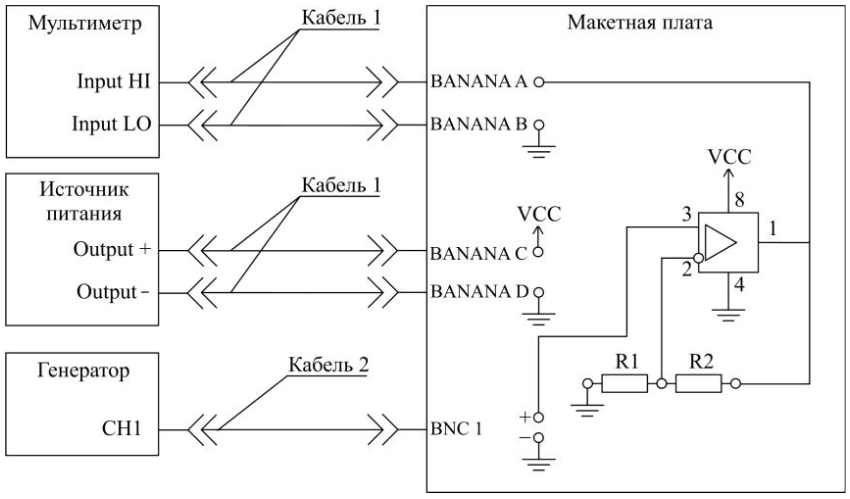
\includegraphics[width=\textwidth]{scheme2.png}
\end{figure}

\begin{table}[H]
  \begin{tabularx}{\textwidth}{|p{4cm}|p{5cm}|C|C|}
    \hline
    Генератор сигналов & $U_{\text{DC}}$: $0.2$ В & \multicolumn{2}{|p{6cm}|}{\centering Внешняя нагрузка: HighZ} \\
    \hline
    Источник питания & Выходное напряжение: $5$ В & \multicolumn{2}{|p{6cm}|}{\centering Выходной ток: $0.1$ А } \\
    \hline
    Мультиметр & Диапазон: $2$ В & $\nu: 2.5$ изм/с & $R_U$: $10$ МОм \\
    \hline    
    \multicolumn{4}{|p{16cm}|}{\centering Многократное измерение выходного напряжения} \\
    \hline
    \directlua{
      tex.print("\\multicolumn{2}{|p{9cm}|}{ Количество элементов} & \\multicolumn{2}{p{6cm}|}{ \\centering $" .. n5 .. "$} \\\\ \\hline")
      tex.print("\\multicolumn{2}{|p{9cm}|}{ Минимальное значение, В } & \\multicolumn{2}{p{6cm}|}{ \\centering $" .. value_with_mantice(find_min(E3data), 6, -1, 0) .. "$} \\\\ \\hline")
      tex.print("\\multicolumn{2}{|p{9cm}|}{ Максимальное значение, В } & \\multicolumn{2}{p{6cm}|}{ \\centering $" .. value_with_mantice(find_max(E3data), 6, -1, 0) .. "$} \\\\ \\hline")
      tex.print("\\multicolumn{2}{|p{9cm}|}{ Среднеквадратичное отклонение выборки, В } & \\multicolumn{2}{p{6cm}|}{ \\centering $" .. value_with_mantice(S5, 5, -5, 0) .. "$} \\\\ \\hline")
      tex.print("\\multicolumn{2}{|p{9cm}|}{ Выборочное среднее арифметическое, В } & \\multicolumn{2}{p{6cm}|}{ \\centering $" .. value_with_mantice(m5, 6, -1, 0) .. "$} \\\\ \\hline")
      tex.print("\\multicolumn{2}{|p{9cm}|}{ Дисперсия, В$^2$ } & \\multicolumn{2}{p{6cm}|}{ \\centering $" .. value_with_mantice(D5, 5, 0, 0) .. "$} \\\\ \\hline")
      tex.print("\\multicolumn{2}{|p{9cm}|}{ Коэффициент асимметрии} & \\multicolumn{2}{p{6cm}|}{ \\centering $" .. value_with_mantice(A5, 5, -1, 0) .. "$} \\\\ \\hline")
      tex.print("\\multicolumn{2}{|p{9cm}|}{ Коэффициент куртозиса} & \\multicolumn{2}{p{6cm}|}{ \\centering $" .. value_with_mantice(k5 - 3, 5, -1, 0) .. "$} \\\\ \\hline")
    }
  \end{tabularx}
\end{table}

\subsubsection{Построение Гистограммы и выдвижение гипотезы распределения}

Предположим, что данные подчиняются нормальному распределению. Строим гистограмму
распределения результатов измерений выходного напряжения $U_\text{вых}$ и
теоретическую кривую нормального распределения с помощью формулы (\ref{normal_distribution}),
используя в качестве параметров $\mu$ по формуле (\ref{normal_distribution:mean})
\begin{equation*}
  \mu = \overline{x} = \frac{1}{\directlua{tex.print(n5)}} \sum_{i=1}^{\directlua{tex.print(n5)}} x_i = \directlua{tex.print(value_with_mantice(m5, 6, 4, 3))} \text{ В}  
\end{equation*}
и $\sigma$ по формуле (\ref{normal_distribution:stddev})
\begin{equation*}
  \sigma = \tilde{\sigma} = \sqrt{\frac{1}{\directlua{tex.print(n5)} - 1} \sum_{i=1}^{\directlua{tex.print(n5)}} (x_i - \directlua{tex.print(value_with_mantice(m5, 6, 4, 3))})^2} = \directlua{tex.print(value_with_mantice(S5, 5, -1, 3))} \text{ В}  
\end{equation*}

\begin{figure}[H]
\centering
\begin{tikzpicture}
\begin{axis}[
    width=0.95\textwidth,
    height=0.55\textwidth,
    grid=both,
    major grid style={line width=0.4pt, draw=gray!45},
    minor grid style={line width=0.2pt, draw=gray!20},
    xlabel={Оценка математического ожидания, В},
    ylabel={Плотность вероятности},
    title={Гистограмма распределения результатов измерений $U_\text{вых}$},
    xmin=\directlua{
      if -E3histogram_interval_coords[1].x > E3histogram_interval_coords[r5 + 1].x then 
        tex.print(E3histogram_interval_coords[1].x * 1.05)
      else 
        tex.print(-E3histogram_interval_coords[r5 + 1].x * 1.05)
      end  
    },
    xmax=\directlua{
      if -E3histogram_interval_coords[1].x > E3histogram_interval_coords[r5 + 1].x then 
        tex.print(-E3histogram_interval_coords[1].x * 1.05)
      else 
        tex.print(E3histogram_interval_coords[r5 + 1].x * 1.05)
      end 
    },
    ymin=0,
    ymax=\directlua{
      local maxy = 0
      for i, v in ipairs(E3histogram_interval_coords) do
        if type(v.y) == "number" and v.y > maxy then maxy = v.y end
      end
      if not (maxy == maxy) or maxy == 0 then maxy = 1 end
      tex.print(maxy * 1.2)
    },
    minor tick num=1,
    tick align=outside,
    legend style={
        at={(0.0,1.0)},
        anchor=north west,
        draw=none,
        fill=white,
        fill opacity=0.25,
        text opacity=1
    },
]
% Гистограмма.
% Используется плотность: h_i = N_i / (n l)
\addplot+[
    ybar interval,
    draw=black,
    fill=gray!45,
    fill opacity=0.75,
    area legend,
] coordinates {
\directlua{
  for i, v in ipairs(E3histogram_interval_coords) do
    tex.print("(" .. v.x .. ", " .. v.y .. ") ")
  end
}
};

\addplot[
    black,
    thick,
    smooth,
    samples=200,
    domain=\directlua{
      if -E3histogram_interval_coords[1].x > E3histogram_interval_coords[r5 + 1].x then 
        tex.print(E3histogram_interval_coords[1].x * 1.05)
      else 
        tex.print(-E3histogram_interval_coords[r5 + 1].x * 1.05)
      end  
    }:\directlua{
      if -E3histogram_interval_coords[1].x > E3histogram_interval_coords[r5 + 1].x then 
        tex.print(-E3histogram_interval_coords[1].x * 1.05)
      else 
        tex.print(E3histogram_interval_coords[r5 + 1].x * 1.05)
      end 
    },
] {
  1 / (\directlua{tex.print(S5)} * sqrt(2*pi)) * exp(-0.5 * (x / \directlua{tex.print(S5)})^2)
};
\legend{\small Эмпирические данные, \small Нормальное распределение}
\end{axis}
\end{tikzpicture}
\label{fig:gistogram-u}
\end{figure}

\subsubsection{Проверка гипотезы распределения}

Проверяем гипотезу о том, что данные подчиняются нормальному распределению, с помощью критерия
$\chi^2$ Пирсона (\ref{chi2:critical})
\begin{equation*}
  \chi^2 = \directlua{tex.print(value_with_mantice(chi25, 3, 0, 0))} < \chi^2_{0.05, 4} = \directlua{tex.print(chi2critical)}
\end{equation*}
так как критерий выполняется, то гипотеза о том, что данные подчиняются нормальному 
распределению, не отвергается.

\subsubsection{Оценка доверительной погрешности}

Найдём средне-квадратическую ошибку среднего арифметического по формуле (\ref{normal_distribution:stddev:mean})
\begin{equation*}
  \tilde{\sigma}_{\overline{x}} = \frac{\directlua{tex.print(value_with_mantice(S5, 5, -5, 0))}}{\sqrt{\directlua{tex.print(n5)}}} = \directlua{tex.print(value_with_mantice(Sm5, 5, -6, 0))} \text{ В} 
\end{equation*}

Так как данные подчиняются нормальному распределению, то для оценки доверительной
погрешности можно использовать формулу (\ref{student:confidence})
\begin{equation*}
  \varepsilon(\alpha) = \pm t_{0.05, \directlua{tex.print(n5 - 1)}} \cdot \tilde{\sigma}_{\overline{x}} = \pm \directlua{tex.print(value_with_mantice(t5, 5, 0, 0))} \cdot \directlua{tex.print(value_with_mantice(Sm5, 5, -6, 0))} = \pm \directlua{tex.print(value_with_mantice(delta_m5, 5, 0, 0))} \text{ В}
\end{equation*}

Берём приборную погрешность мультиметра как неисключаемую систематическую погрешность
\begin{equation*}
  \Theta_\Sigma = \Theta_U = \pm(0.020\% \cdot \directlua{tex.print(value_with_mantice(m5, 6, -1, 0))} + 0.003\% \cdot 2) = \pm \directlua{tex.print(value_with_mantice(Theta5, 5, 0, 0))} \text{ В}
\end{equation*}

Погрешность оценки измеряемой величины $U_\text{вых}$ по формуле (\ref{delta:confidence})
\begin{equation*}
  \begin{aligned}
    \tilde{\sigma}_\Theta &= \frac{\directlua{tex.print(value_with_mantice(Theta5, 5, 0, 0))}}{\sqrt{3}} = \directlua{tex.print(value_with_mantice(Stheta5, 5, 0, 0))} \text{ В}  \\ 
    K &= \directlua{tex.print("\\frac{" .. value_with_mantice(delta_m5, 5, 0, 0) .. "+" .. value_with_mantice(Theta5, 5, 0, 0) .. "}{" .. value_with_mantice(Sm5, 5, 0, 0) .. "+" .. value_with_mantice(Stheta5, 5, 0, 0) .. "} = " .. value_with_mantice(K5, 5, 0, 0))} \\ 
    \tilde{\sigma}_\Sigma &= \sqrt{(\directlua{tex.print(value_with_mantice(Sm5, 5, 0, 0))})^2 + (\directlua{tex.print(value_with_mantice(Stheta5, 5, 0, 0))})^2} = \\
    &= \directlua{tex.print(value_with_mantice(Ssum5, 5, 0, 0))} \text{ В} 
  \end{aligned}
\end{equation*}
\begin{equation*}
  \Delta(\alpha) = \pm \directlua{tex.print(value_with_mantice(K5, 5, 0, 0))} \cdot \directlua{tex.print(value_with_mantice(Ssum5, 5, 0, 0))} = \pm \directlua{tex.print(value_with_mantice(delta5, 5, -4, 0))} \text{ В}
\end{equation*}

\subsubsection{Результат измерения}

Запишем результат измерения с учётом значащих цифр по формуле (\ref{final:result})
\begin{equation*}
  U_\text{вых} = (\CalcFive{\directlua{tex.print(value_with_mantice(m5, 6, -1, 0))}} \pm \directlua{tex.print(value_with_mantice(delta5, 2, -4, 0))}) \text{ В}
\end{equation*}

\subsection{Многократное измерение выходного напряжения через резисторы $R_1$, $R_2$
и $U_\text{DC}$}

\subsubsection{Схема и протокол измерительного эксперимента}

Напряжение $U_\text{вых}$ измеряется через резисторы $R_1$, $R_2$ и $U_\text{DC}$, так что измерение
является косвенным, поэтому используется иная методика обработки результатов измерений.

Измерения проводились в разное время, так что коэффициент корреляции между измерениями 
$R_1$, $R_2$ и $U_\text{DC}$ равен нулю.

Зависимость $U_\text{вых}$ от $R_1$, $R_2$ и $U_\text{DC}$ согласно формуле (\ref{amplifier:output}) 
\begin{equation*}
  U_\text{вых}(R_1, R_2, U_\text{DC}) = \left(1 + \frac{R_2}{R_1}\right) U_\text{DC}
\end{equation*}
является нелинейной, так что требуется провести линеризацию функции
$U_\text{вых}(R_1, R_2, U_\text{DC})$.

\subsubsection{Оценка величины}

Оценим выходное напряжение измерительного преобразователя по формуле (\ref{amplifier:output})
\begin{equation*}
  U_\text{вых} = \left(1 + \frac{R_2}{R_1}\right)U_\text{вх}
\end{equation*}
где в качестве $U_\text{вх}$ берётся оценка напряжения генератора $U_{DC}$, полученная
в первом измерительном эксперименте, а в качестве $R_1$ и $R_2$ берутся оценки сопротивлений,
полученные во втором измерительном эксперименте.

Тогда
\begin{equation*}
  \begin{aligned}
    U_{\text{вых}} 
    &= \left(1 + \frac{\overline{R}_2}{\overline{R}_1}\right)\overline{U}_{DC} = \\
    &= \left(1 + \frac{\directlua{tex.print(value_with_mantice(m31, 6, 4, 0))}}
    {\directlua{tex.print(value_with_mantice(m21, 6, 4, 0))}}\right)
    \cdot \directlua{tex.print(value_with_mantice(m11, 6, -1, 0))} = \\
    &= \directlua{tex.print(value_with_mantice(m6, 6, -1, 0))} \text{ В}
  \end{aligned}
\end{equation*}

Коэффициент усиления измерительного преобразователя по формуле (\ref{amplifier:gain})
\begin{equation*}
  K = 1 + \frac{R_2}{R_1}
  =
  1 + \frac{\directlua{tex.print(value_with_mantice(m31, 6, 4, 0))}}
  {\directlua{tex.print(value_with_mantice(m21, 6, 4, 0))}}
  =
  \directlua{tex.print(value_with_mantice(dUdU6, 6, 0, 0))}
\end{equation*}

\subsubsection{Оценка случайно состовляющей погрешности}

Так как зависимость $U_\text{вых}(U_\text{вх}, R_1, R_2)$ является нелинейной, используем
формулу линеаризации (\ref{nonlinear:indirect}). Для этого найдём частные производные:
\begin{equation*}
  \frac{\partial U_\text{вых}}{\partial U_\text{вх}}
  =
  1 + \frac{R_2}{R_1}
\end{equation*}
\begin{equation*}
  \frac{\partial U_\text{вых}}{\partial R_1}
  =
  -\frac{U_\text{вх}R_2}{R_1^2}
\end{equation*}
\begin{equation*}
  \frac{\partial U_\text{вых}}{\partial R_2}
  =
  \frac{U_\text{вх}}{R_1}
\end{equation*}

Подставим значения
\begin{equation*}
  \begin{aligned}
    \frac{\partial U_\text{вых}}{\partial U_\text{вх}}
    &=
    1 + \frac{\directlua{tex.print(value_with_mantice(m31, 6, 4, 0))}}
    {\directlua{tex.print(value_with_mantice(m21, 6, 4, 0))}}
    =
    \directlua{tex.print(value_with_mantice(dUdU6, 6, 0, 0))}
    \\
    \frac{\partial U_\text{вых}}{\partial R_1}
    &=
    -\frac{\directlua{tex.print(value_with_mantice(m11, 6, -1, 0))}\cdot
    \directlua{tex.print(value_with_mantice(m31, 6, 4, 0))}}
    {\left(\directlua{tex.print(value_with_mantice(m21, 6, 4, 0))}\right)^2}
    =
    \directlua{tex.print(value_with_mantice(dUdR16, 6, 0, 0))}\ \frac{\text{В}}{\text{Ом}}
    \\
    \frac{\partial U_\text{вых}}{\partial R_2}
    &=
    \frac{\directlua{tex.print(value_with_mantice(m11, 6, -1, 0))}}
    {\directlua{tex.print(value_with_mantice(m21, 6, 4, 0))}}
    =
    \directlua{tex.print(value_with_mantice(dUdR26, 6, 0, 0))}\ \frac{\text{В}}{\text{Ом}}
  \end{aligned}
\end{equation*}

Среднеквадратическое отклонение косвенной оценки выходного напряжения по формуле 
(\ref{nonlinear:indirect})
\begin{equation*}
  \begin{aligned}
    \tilde{\sigma}_{U_\text{вых}}
    &=
    \sqrt{
    \left(\frac{\partial U_\text{вых}}{\partial U_\text{вх}}\right)^2
    \tilde{\sigma}_{\overline{U}_{DC}}^2
    +
    \left(\frac{\partial U_\text{вых}}{\partial R_1}\right)^2
    \tilde{\sigma}_{\overline{R}_1}^2
    +
    \left(\frac{\partial U_\text{вых}}{\partial R_2}\right)^2
    \tilde{\sigma}_{\overline{R}_2}^2
    }
    =
    \\
    &=
    \sqrt{
    \begin{aligned}
      \left(\directlua{tex.print(value_with_mantice(dUdU6, 6, 0, 0))}\right)^2
      \left(\directlua{tex.print(value_with_mantice(Sm1, 5, 0, 0))}\right)^2
      +
      \left(\directlua{tex.print(value_with_mantice(dUdR16, 5, 0, 0))}\right)^2
      \left(\directlua{tex.print(value_with_mantice(Sm2, 5, 0, 0))}\right)^2 + \\
      +
      \left(\directlua{tex.print(value_with_mantice(dUdR26, 5, 0, 0))}\right)^2
      \left(\directlua{tex.print(value_with_mantice(Sm3, 5, 0, 0))}\right)^2
    \end{aligned}
    }
    =
    \\
    &=
    \directlua{tex.print(value_with_mantice(Sm6, 5, -6, 0))}\text{ В}
  \end{aligned}
\end{equation*}

Квантиль нормального распределения для доверительной вероятности $\alpha = 0.95$ равен
$z_{0.975} = 1.96$, так что доверительная погрешность оценки
по формуле (\ref{nonlinear:indirect})
\begin{equation*}
  \varepsilon_{U_\text{вых}}(\alpha)
  =
  \pm \directlua{tex.print(value_with_mantice(z6, 3, 0, 0))}\cdot
  \directlua{tex.print(value_with_mantice(Sm6, 5, 0, 0))}
  =
  \pm \directlua{tex.print(value_with_mantice(delta_m6, 5, -6, 0))}\text{ В}
\end{equation*}

\subsubsection{Оценка систематической погрешности}

Суммарную неисключаемую систематическую погрешность косвенного измерения оцениваем
по формуле (\ref{nonlinear:indirect})
\begin{equation*}
  \begin{aligned}
    \Theta_{U_\text{вых}}
    &=
    \sqrt{
    \left(\frac{\partial U_\text{вых}}{\partial U_\text{вх}}\right)^2
    \Theta_{U_{DC}}^2
    +
    \left(\frac{\partial U_\text{вых}}{\partial R_1}\right)^2
    \Theta_{R_1}^2
    +
    \left(\frac{\partial U_\text{вых}}{\partial R_2}\right)^2
    \Theta_{R_2}^2
    }
    =
    \\
    &=
    \sqrt{
    \begin{aligned}
      \left(\directlua{tex.print(value_with_mantice(dUdU6, 6, 0, 0))}\right)^2
      \left(\directlua{tex.print(value_with_mantice(Theta1, 5, 0, 0))}\right)^2
      +
      \left(\directlua{tex.print(value_with_mantice(dUdR16, 5, 0, 0))}\right)^2
      \left(\directlua{tex.print(value_with_mantice(Theta2, 5, 0, 0))}\right)^2 + \\
      +
      \left(\directlua{tex.print(value_with_mantice(dUdR26, 5, 0, 0))}\right)^2
      \left(\directlua{tex.print(value_with_mantice(Theta3, 5, 0, 0))}\right)^2
    \end{aligned}
    }
    =
    \\
    &=
    \directlua{tex.print(value_with_mantice(Theta6, 5, -4, 0))}\text{ В}
  \end{aligned}
\end{equation*}

Погрешность оценки косвенно измеряемой величины $U_\text{вых}$ по формуле 
(\ref{nonlinear:indirect:confidence})
\begin{equation*}
  \begin{aligned}
    \tilde{\sigma}_\Theta
    &=
    \frac{\directlua{tex.print(value_with_mantice(Theta6, 5, -4, 0))}}{\sqrt{3}}
    =
    \directlua{tex.print(value_with_mantice(Stheta6, 5, -4, 0))}\text{ В}
    \\
    K
    &=
    \directlua{tex.print("\\frac{" .. value_with_mantice(delta_m6, 5, -6, 0) .. "+" .. value_with_mantice(Theta6, 5, -4, 0) .. "}{" .. value_with_mantice(Sm6, 5, -6, 0) .. "+" .. value_with_mantice(Stheta6, 5, -4, 0) .. "} = " .. value_with_mantice(K6, 5, 0, 0))}
    \\
    \tilde{\sigma}_\Sigma
    &=
    \sqrt{
    \left(\directlua{tex.print(value_with_mantice(Sm6, 5, -6, 0))}\right)^2
    +
    \left(\directlua{tex.print(value_with_mantice(Stheta6, 5, -4, 0))}\right)^2
    }
    =
    \directlua{tex.print(value_with_mantice(Ssum6, 5, -4, 0))}\text{ В}
  \end{aligned}
\end{equation*}
\begin{equation*}
  \Delta_{U_\text{вых}}(\alpha)
  =
  \pm \directlua{tex.print(value_with_mantice(K6, 5, 0, 0))}\cdot
  \directlua{tex.print(value_with_mantice(Ssum6, 5, -4, 0))}
  =
  \pm \directlua{tex.print(value_with_mantice(delta6, 5, -4, 0))}\text{ В}
\end{equation*}

\subsubsection{Результат измерения}

Запишем результат косвенного измерения с учётом значащих цифр по формуле
(\ref{final:result})
\begin{equation*}
  U_{\text{вых}}
  =
  \left(
  \CalcFive{\directlua{tex.print(value_with_mantice(m6, 6, -1, 0))}}0
  \pm
  \directlua{tex.print(value_with_mantice(delta6, 2, -4, 0))}
  \right)\text{ В}
\end{equation*}

\fancyhead[L]{Выводы}

\section{Выводы}

В ходе выполнения лабораторной работы была достигнута цель работы:
были поставлены многократные прямые и косвенные измерения, выполнена
статистическая обработка выборок, а также получены оценки действительных
значений измеряемых величин с последующей оценкой случайных,
систематических и суммарных погрешностей.

В первом измерительном эксперименте было выполнено многократное измерение
напряжения постоянного тока на выходе генератора сигналов. После внесения
методической поправки, связанной с влиянием входного сопротивления мультиметра,
получено
\begin{equation*}
  U_{DC}
  =
  \left(
  \directlua{tex.print(value_with_mantice(m11, 5, -1, 0))}
  \pm
  \directlua{tex.print(value_with_mantice(delta1, 2, -5, 0))}
  \right)\text{ В}
\end{equation*}
при доверительной вероятности $\alpha = 0.95$. Количество измерений составило
\begin{equation*}
  n = \directlua{tex.print(n1)}
\end{equation*}

Для оценки доверительной границы случайной погрешности
использовался критерий Стьюдента.

Во втором измерительном эксперименте были выполнены многократные измерения
сопротивлений резисторов $R_1$ и $R_2$ по двухпроводной схеме. Для резистора
$R_1$ получено
\begin{equation*}
  R_1
  =
  \left(
  \directlua{tex.print(value_with_mantice(m21, 6, 4, 0))}
  \pm
  \directlua{tex.print(value_with_mantice(delta2, 2, 0, 0))}
  \right)\text{ Ом}
\end{equation*}
Для резистора $R_2$ получено
\begin{equation*}
  R_2
  =
  \left(
  \directlua{tex.print(value_with_mantice(m31, 4, 4, 0))}
  \pm
  \directlua{tex.print(value_with_mantice(delta3, 2, 1, 0))}
  \right)\text{ Ом}
\end{equation*}
Доверительная вероятность была выполнена по формуле Чёбышёва для
обеих выборок.

Также была выполнена косвенная оценка сопротивления последовательного
соединения резисторов $R_1$ и $R_2$ по формуле
\begin{equation*}
  R_\Sigma = R_1 + R_2
\end{equation*}
В результате получено
\begin{equation*}
  R_\Sigma
  =
  \left(
  \directlua{tex.print(value_with_mantice(m4, 5, 4, 0))}
  \pm
  \directlua{tex.print(value_with_mantice(delta4, 2, 1, 0))}
  \right)\text{ Ом}
\end{equation*}
Так как выборки $R_1$ и $R_2$ получены для разных физических элементов в разный момент и
рассматриваются как независимые.

В третьем измерительном эксперименте было выполнено многократное измерение
выходного напряжения масштабирующего измерительного преобразователя на базе
операционного усилителя. Для прямого многократного измерения получено
\begin{equation*}
  U_{\text{вых, прям}}
  =
  \left(
  \directlua{tex.print(value_with_mantice(m5, 6, -1, 0))}
  \pm
  \directlua{tex.print(value_with_mantice(delta5, 2, -4, 0))}
  \right)\text{ В}
\end{equation*}
при количестве измерений
\begin{equation*}
  n = \directlua{tex.print(n5)}
\end{equation*}

После этого была выполнена косвенная оценка выходного напряжения
масштабирующего измерительного преобразователя по формуле
\begin{equation*}
  U_{\text{вых, кос}}
  =
  \left(1 + \frac{R_2}{R_1}\right)U_{DC}
\end{equation*}
В результате получено
\begin{equation*}
  U_{\text{вых, кос}}
  =
  \left(
  \directlua{tex.print(value_with_mantice(m6, 6, -1, 0))}
  \pm
  \directlua{tex.print(value_with_mantice(delta6, 2, -4, 0))}
  \right)\text{ В}
\end{equation*}
Границы прямого измерения выходного напряжения
\begin{equation*}
  U_{\text{вых, прям}}
  \in
  \left[
  \directlua{tex.print(value_with_mantice(UoutDirectMin, 6, -1, 0))};
  \directlua{tex.print(value_with_mantice(UoutDirectMax, 6, -1, 0))}
  \right]\text{ В}
\end{equation*}
Границы косвенного измерения выходного напряжения
\begin{equation*}
  U_{\text{вых, кос}}
  \in
  \left[
  \directlua{tex.print(value_with_mantice(UoutIndirectMin, 6, -1, 0))};
  \directlua{tex.print(value_with_mantice(UoutIndirectMax, 6, -1, 0))}
  \right]\text{ В}
\end{equation*}
По результатам сравнения доверительные интервалы
\directlua{
  if UoutIntervalsCross then
    tex.print("прямого и косвенного измерений пересекаются")
  else
    tex.print("прямого и косвенного измерений не пересекаются")
  end
}
. Это позволяет сделать вывод о том, насколько идеальная модель
неинвертирующего усилителя согласуется с результатом прямого многократного
измерения. Если интервалы не пересекаются, то расхождение может быть связано
с неучтенными систематическими составляющими, влиянием реальной схемы
операционного усилителя, режимом питания, нагрузкой или отличием реального
коэффициента усиления от расчетного.

Таким образом, в ходе лабораторной работы были получены выборки многократных
измерений, построены гистограммы экспериментальных распределений, проверены
гипотезы о виде распределений с помощью критерия Пирсона, оценены случайные
и неисключенные систематические составляющие погрешности, а также рассчитаны
суммарные погрешности прямых и косвенных измерений. Полученные результаты
показывают, что многократные измерения позволяют оценить разброс показаний
и уменьшить влияние случайной составляющей за счет использования среднего
арифметического, однако итоговая точность результата в значительной степени
ограничивается приборной и методической составляющими погрешности.

\fancyhead[L]{Список используемой литературы}

\section{Список используемой литературы}

\begin{enumerate}
  \item Калеев Д. В. Метрология и электрорадиоизмерения: лабораторный практикум. М.: МИЭТ, 2025. 184 с.
  \item ГОСТ Р 8.736--2011. Государственная система обеспечения единства измерений. Измерения прямые многократные. Методы обработки результатов измерений. Основные положения.
  \item РМГ 29--2013. Государственная система обеспечения единства измерений. Метрология. Основные термины и определения.
  \item RIGOL Technologies. DM3058/DM3058E Digital Multimeter. User's Guide.
  \item RIGOL Technologies. DG1000Z Series Function/Arbitrary Waveform Generator. User's Guide.
\end{enumerate}


\end{document}